\documentclass[11pt,openany,a4paper]{article}
\usepackage{amsmath, amsfonts, amssymb, amsthm}
\usepackage{tikz, pgfplots, tkz-euclide,calc}
    \usetikzlibrary{patterns,decorations,shapes.arrows,intersections, pgfplots.fillbetween}
    \tikzset{Arrow Style/.style={text=black, font=\boldmath}}
    \newcommand{\tikzmark}[1]{%
        \tikz[overlay, remember picture, baseline] \node (#1) {};%
    }

    \newcommand*{\XShift}{0.5em}
    \newcommand*{\YShift}{0.5ex}

    \NewDocumentCommand{\DrawArrow}{s O{} m m m}{%
        \begin{tikzpicture}[overlay,remember picture]
            \draw[->, thick, Arrow Style, #2] 
                    ($(#3.west)+(\XShift,\YShift)$) -- 
                    ($(#4.east)+(-\XShift,\YShift)$)
            node [midway,above] {#5};
        \end{tikzpicture}%
    }
    \newcommand{\AxisRotator}[1][rotate=0]{%
    \tikz [x=0.25cm,y=0.60cm,line width=0.15ex,-stealth,#1,solid] \draw (0,0) arc (330:30:0.5 and 0.5);%
    }
\usepackage{fancyhdr}
\usepackage{enumerate,enumitem}
\usepackage{cancel}
\usepackage{polynom}
\makeatletter
\patchcmd{\pld@ArrangeResult}{\bigr)}{
    \,\tikz[overlay]{
        \coordinate (A) at (0,-3pt);
        \coordinate (B) at (0,\normalbaselineskip-0.8pt);
        \draw (A) to[in=-40, out=40, looseness=1] (B);
    }
}{}{}
\makeatother
\makeatletter
\patchcmd{\pld@ArrangeResult}{\tw@-\pld@maxcol}{
  \tw@-\pld@maxcol
}{}{}
\makeatother
\usepackage{varwidth}
\usepackage{hyperref}
\hypersetup{
    colorlinks=true,
    linkcolor=blue,
    filecolor=magenta,      
    urlcolor=cyan,
    }

% TAMBAHKAN PACKAGE SENDIRI KALAU KURANG

\usepackage{geometry}
\geometry{
	total = {160mm, 237mm},
	left = 18mm,
	right = 13mm,
	top = 30mm,
	bottom = 30mm,
}


\pagestyle{fancy}
\fancypagestyle{problems}{
  \fancyhead{}
  \fancyfoot{}
  \fancyhead[r]{}
  \fancyhead[l]{\fbox{\large{\textbf{SKPB - ITS}}}}
  \renewcommand{\headrulewidth}{0pt}
  \renewcommand{\footrulewidth}{0pt}
}

\renewcommand{\headrulewidth}{0pt}
\renewcommand{\footrulewidth}{0pt}
\renewcommand{\hrulefill}{\leavevmode\leaders\hrule height 2pt\hfill\kern0pt}


\fancypagestyle{solution}{
  \pagestyle{fancy}
  \newpage
  \fancyhead[L]{\textit{Solution By: \hyperlink{https://github.com/TetewHeroez}{Tetew Heroez}}}
  % \fancyfoot[R]{\animategraphics[autoplay,loop,width=0.1\textwidth]{15}{Kuru Kuru Herta/kuru kuru-}{0}{5}}
  \fancyfoot{}
  \renewcommand{\headrulewidth}{1pt}
}

\newcommand{\Hrule}{\stackrel{\text{\raisebox{1.5pt}{\textcircled{\raisebox{-.9pt} {L}}}}}{=}}

\definecolor{Acolor}{RGB}{134, 218, 200} 

\begin{document}
\pagestyle{problems}
    \begin{center}
	{\underline{\textbf{\MakeUppercase{Evaluasi Akhir Semester Bersama Genap 2023/2024}}}}
    \end{center}

    \begin{center}
	\begin{tabular}{lcl}
		Mata kuliah/SKS & : & Kalkulus 2 ( SM234201 ) / 3 SKS\\
		Hari, Tanggal & : & Rabu, 26 Juni 2024\\
		Waktu & : & 07.00-08.40 WIB (100 menit)\\
		Sifat & : & Tertutup\\
		Kelas & : & 1-13, 101
	\end{tabular}
    \end{center}
	
    \noindent\rule{\textwidth}{2.pt}
	
    \setlength{\parindent}{5pt}
    \par Diberikan 5 soal, dengan bobot nilai masing-masing soal sama dan boleh dikerjakan tidak berurutan.
    \setlength{\parindent}{5pt}
    \centering{Tuliskan: Nama, NRP, dan Nomor Kelas pada lembar jawaban Anda.}
    \setlength{\parindent}{5pt}
    {\small
    \par \textbf{\MakeUppercase{Dilarang membawa/menggunakan kalkulator dan alat komunikasi}}
    \centering{\textbf{\MakeUppercase{dilarang memberikan/menerima jawaban selama ujian}}}}
    \par \centering{\textbf{"Setiap tindak kecurangan akan mendapat sanksi akademik."}}
	
    \noindent\rule{\textwidth}{2.pt}
	
% SOAL DI SINI YAA
\begin{enumerate}
    \item Dapatkan luas daerah yang dibatasi oleh \( x = y^2 \) dan \( 2y + x = 3 \).

    \item Gambarkan daerah yang dibatasi oleh kurva-kurva \( y = \sqrt{x} \), \( y = 2 \), dan \( x = 0 \), kemudian dapatkan volume benda putar jika daerah tersebut diputar pada garis \( x = -2 \).

    \item Diberikan persamaan parametrik \( x = t^2 + 1 \), \( y = t \), \( 0 \leq t \leq 5 \).
    \begin{enumerate}
        \item Buatlah sketsa kurva tersebut dengan mengeliminasi parameter \( t \).
        \item Dapatkan persamaan garis singgung dari persamaan parametrik tersebut saat \( t = \frac{1}{2} \).
    \end{enumerate}

    \item Dapatkan luas daerah dari irisan kardioida \( r = 2 - 2 \cos \theta \) dan kardioida \( r = 2 + 2 \cos \theta \).

    \item Dapatkan lima suku pertama polinomial Maclaurin untuk fungsi \( f(x) = e^{-x^2} \).
\end{enumerate}
	
    \fancyfoot{
    \hrulefill\textbf{ Selamat Mengerjakan }\hrulefill

    \begin{center}
	    ``\textit{Jujur adalah kunci kesuksesan}''
    \end{center}}

    \newpage
    \pagestyle{solution}
    {\centering\textbf{SOLUSI}}
    
    \begin{enumerate}
      \item Karena batas daerahnya belum diketahui, maka seharusnya batas daerah/luasnya didapatkan melalui titik potong kedua kurva tersebut.
        \begin{align*}
            y^2 &= 3 - 2y \\
            y^2 + 2y - 3 &= 0 \\
            (y+3)(y-1) &= 0 \\
            y=-3 \quad&\vee\quad y=1 
        \end{align*}
        Ilustrasi daerah yang dibatasi oleh kedua kurva tersebut adalah sebagai berikut:
        \begin{center}
          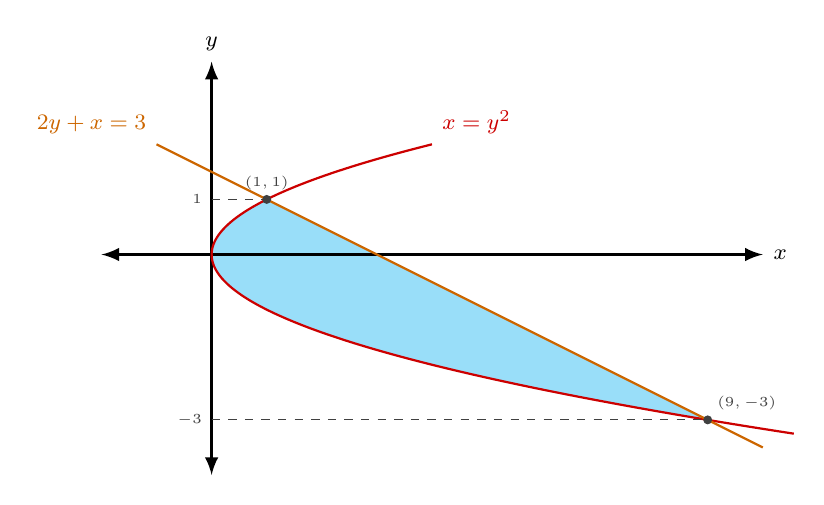
\begin{tikzpicture}[scale=0.7]
          \def\fy{\y*\y}
          \def\gy{3-2*\y}
          %shading
          \fill[domain=-3:1,smooth,samples=100,variable=\y, cyan!40] plot ({\fy},{\y})--(9,-3);

          %axes
          \draw[latex-latex,very thick] (-2,0)--(10,0) node [right] {\footnotesize$x$};
          \draw[latex-latex,very thick] (0,-4)--(0,3.5) node [above] {\footnotesize$y$};

          %graphs
          \draw[domain=-3.25:2,smooth,samples=120,variable=\y, red!80!black, thick] plot ({\fy},{\y}) node [above right] {\footnotesize$x=y^2$};
          \draw[domain=-3.5:2,smooth,variable=\y, thick, orange!80!black] plot ({\gy},{\y}) node [above left] {\footnotesize$2y+x=3$};

          %intersection points
          \draw[fill=black,darkgray] (9,-3) circle (2pt) node [above right] {\tiny$(9,-3)$};
          \draw[fill=black,darkgray] (1,1) circle (2pt) node [above] {\tiny$(1,1)$};
          \draw[darkgray,dashed] (0,-3) node[left] {\tiny$-3$} -- (9,-3);
          \draw[darkgray,dashed] (0,1) node[left] {\tiny$1$} -- (1,1);
          \end{tikzpicture}
        \end{center}
        Perhatikan bahwa perhitungan luas daerah yang diarsir secara umum dapat dilakukan dengan dua cara yang diilustrasikan pada gambar berikut
      \begin{center}
        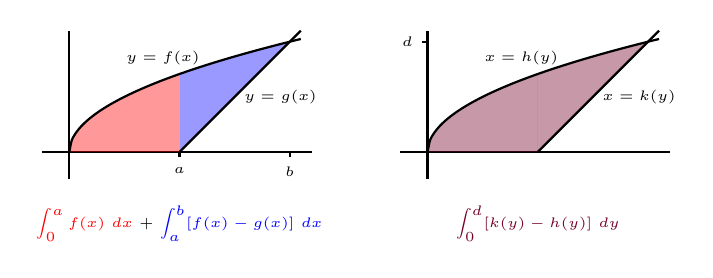
\begin{tikzpicture}[scale=0.7,font=\tiny]
    \def\fxi{sqrt(\x)}
  \draw[thick ](-0.5,0)--(4.4,0);
  \draw[thick ](0,-0.5)--(0,2.2);
  \draw[thick ](2,0)--(2,-0.1);
  \draw[thick](4,0)--(4,-0.1);
  \node[below] at (2,-0.1) {$a$};
  \node[below] at (4,-0.1) {$b$};

  \fill[ domain=0:2,smooth,variable=\x,red, fill opacity=0.4] plot ({\x},{\fxi})--(2,0);
  \fill[ domain=2:4,smooth,variable=\x,blue, fill opacity=0.4] plot ({\x},{\fxi})--(2,0);

  \draw[thick,domain=0:4.2,smooth,samples=100]  plot ({\x},{sqrt(\x)});
  \draw[thick,domain=2:4.2,smooth ]  plot ({\x},{\x-2});
  \node[above,black] at (1.7,1.4) {$y=f(x)$};
  \node[right,black] at (3,1) {$y=g(x)$};
  \node at (2,-1.3) {$\displaystyle \color{red}{\int_0^a f(x) \ dx} \ \color{black}{+} \ \color{blue}{\int_a^b [f(x)-g(x)] \ dx} $}; 
\begin{scope}[xshift=6.5cm]
    \draw[thick](-0.5,0)--(4.4,0);
    \draw[thick](0,-0.5)--(0,2.2);
    \draw[thick](0,2)--(-0.1,2);
    \node[left] at (-0.1,2) {$d$};

    \fill[ domain=0:2,smooth,variable=\x,purple!60!black, fill opacity=0.4]  plot ({\x},{\fxi})--(2,0);
    \fill[ domain=2:4,smooth,variable=\x,purple!60!black, fill opacity=0.4]  plot ({\x},{\fxi})--(2,0);

    \draw[thick,domain=0:4.2,smooth,samples=100]  plot ({\x},{\fxi});
    \draw[thick,domain=2:4.2,smooth ]  plot ({\x},{\x-2});
    \node[above,black] at (1.7,1.4) {$x=h(y)$};
    \node[right,black] at (3,1) {$x=k(y)$};
    \node at (2,-1.3) {$\displaystyle  \color{purple!60!black}{\int_0^d [k(y)-h(y)] \ dy} $}; 
    \end{scope}
    \end{tikzpicture}
      \end{center}
      Dari gambar di atas akan lebih mudah untuk mendapatkan luas daerah jika kita menggunakan integral terhadap \( y \). Daerah yang diarsir diperoleh dari pengintegralan kurva kanan (\( x = 3 - 2y \)) dikurangi kurva kiri (\( x = y^2 \)) dan batas nya mulai dari \( y = -3 \) hingga \( y = 1 \).
        \begin{align*}
            \text{Area} &= \int_{-3}^{1} (3 - 2y - y^2) \, dy \\
            &= \left[ 3y - y^2 - \frac{y^3}{3} \right]_{-3}^{1} \\
            &= \left( 3(1) - (1)^2 - \frac{(1)^3}{3} \right) - \left( 3(-3) - (-3)^2 - \frac{(-3)^3}{3} \right) \\
            &= 3 - 1 - \frac{1}{3} + 9 - 9 + 9 = 11 - \frac{1}{3} = \boxed{\frac{32}{3}}
        \end{align*}
      \item Gambar daerah yang dibatasi oleh kurva-kurva tersebut adalah sebagai berikut:
      \begin{center}
        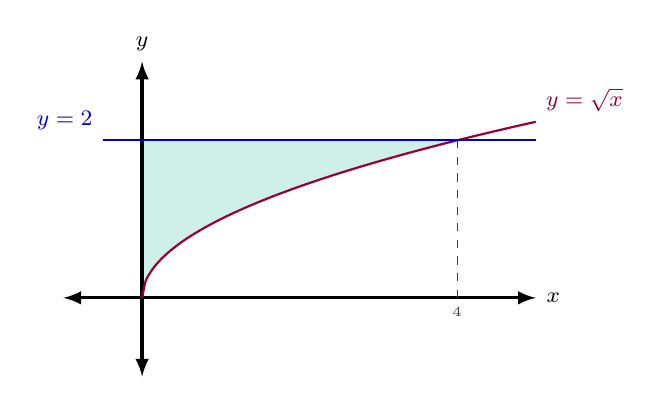
\begin{tikzpicture}[scale=1]
        \def\fx{sqrt(\x)}
        \def\gx{2}
        %shading
        \fill[domain=0:4,smooth,samples=100,variable=\x, Acolor!40] plot ({\x},{\fx})--plot ({\x},{\gx})--(0,2)--(0,0)--cycle;

        %axes
        \draw[latex-latex,very thick] (-1,0)--(5,0) node [right] {\footnotesize$x$};
        \draw[latex-latex,very thick] (0,-1)--(0,3) node [above] {\footnotesize$y$};

        %graphs
        \draw[domain=0:5,smooth,samples=120,variable=\x, purple!80!black, thick] plot ({\x},{\fx}) node [above right] {\footnotesize$y=\sqrt{x}$};
        \draw[domain=5:-0.5,smooth,variable=\x, thick, blue!80!black] plot ({\x},{\gx}) node [above left] {\footnotesize$y=2$};

        %intersection points
        \draw[darkgray,dashed] (4,0) node[below] {\tiny$4$} -- (4,2);
        \end{tikzpicture}
      \end{center}
      Kemudian daerah yang diarsir diputar terhadap garis \( x = -2 \), disini akan digunakan metode cincin silinder. 
      \begin{center}
        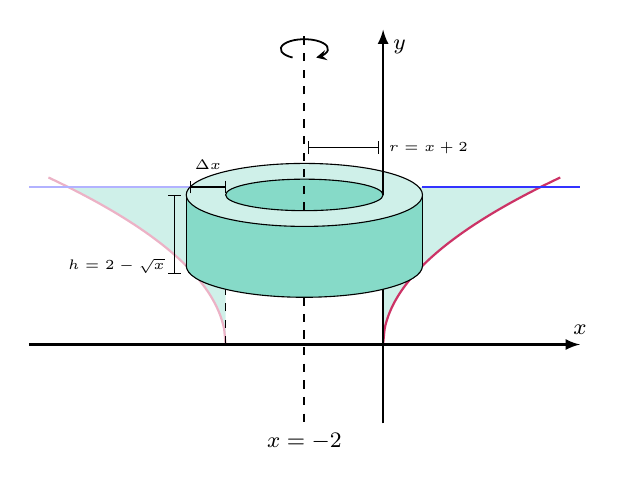
\begin{tikzpicture}[>=latex,x=0.5cm,y=1cm]
            \def\fx{sqrt(\x)}
            \def\gx{2}

            \fill[domain=0:4,smooth,samples=100,variable=\x, Acolor!40] plot ({\x},{\fx})--plot ({\x},{\gx})--(0,2)--(0,0)--cycle;
            \fill[domain=0:4,smooth,samples=100,variable=\x, Acolor!40] plot ({-\x-4},{\fx})--plot ({-\x-4},{\gx})--(-4,2)--(-4,0)--cycle;

            \draw[domain=0:4.5,smooth,samples=120,variable=\x, purple!80, thick] plot ({\x},{\fx});
            \draw[domain=0:4.5,smooth,samples=120,variable=\x, purple!30, thick] plot ({-\x-4},{\fx});
            
            \draw[domain=5:1,smooth,variable=\x, thick, blue!80] plot ({\x},{\gx});
            \draw[domain=-4:-9,smooth,variable=\x, thick, blue!30] plot ({\x},{\gx});

            \draw[fill=Acolor] (-2,1) circle [y radius =.4 , x radius =3];
            \fill[Acolor] (-5,1) rectangle (1,1.9);
            \draw[fill=Acolor!40] (-2,1.9) circle [y radius =.4 , x radius =3];
            \draw[fill=Acolor] (-2,1.9) circle [y radius =.2 , x radius =2];

            \draw[->, thick] (-9,0) -- (5,0) node[above] {\footnotesize $x$};
            \draw[thick] (0,-1) -- (0,0.7);
            \draw[->, thick] (0,1.9) -- (0,4) node[below right]{\footnotesize $y$};
            \draw[dashed] (-4,0) -- (-4,0.7);
            \draw[dashed, thick] (-2,1.7) -- (-2,4) node [midway,pos=0.9] {\AxisRotator[rotate=-90]};
            \draw[dashed, thick] (-2,0.6) -- (-2,-1) node [below] {\footnotesize$x=-2$};

            \draw[very thin] (-5,1.9) -- (-5,1);
            \draw[very thin] (1,1.9) -- (1,1);

            \draw[|-|] (-4.9,2) -- (-4,2) node[midway,above,yshift=0.1cm] {\tiny $\Delta x$};
            \draw[|-|] (-1.9,2.5) -- (-0.1,2.5) node[right] {\tiny $r=x+2$};
            \draw[|-|] (-5.3,1.9) -- (-5.3,0.9) node[left,midway,pos=0.9]  {\tiny $h = 2-\sqrt{x}$};
    \end{tikzpicture}
    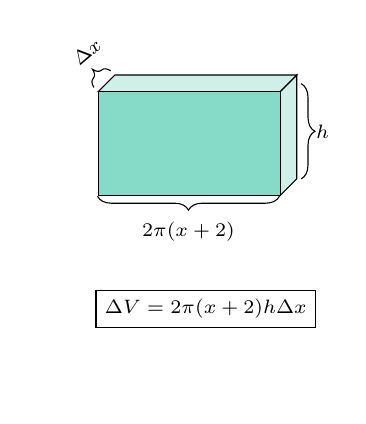
\begin{tikzpicture}[scale=1.1,font=\scriptsize]
            % Connect corners
            \draw (0,0,0) -- (0,0,0.5);
            \draw[fill=Acolor!40] (2.1,0,0) -- (2.1,0,0.5) --(2.1,1.2,0.5)-- (2.1,1.2,0) -- cycle;
            \draw[fill=Acolor!40] (0,1.2,0) -- (0,1.2,0.5) -- (2.1,1.2,0.5) -- (2.1,1.2,0) -- cycle;

            % Draw the top rectangle
            \draw[fill=Acolor] (0,0,0.5) -- (2.1,0,0.5) -- (2.1,1.2,0.5) -- (0,1.2,0.5) -- cycle;

            \draw[black!0] (-1,-1,0) -- (-1,-2.5,0);

            \draw [decorate,decoration={brace,mirror,raise=4ex,amplitude=5pt}] (-0.2,0.35) -- (1.9,0.35) node[midway,yshift=-3em]{$2\pi(x+2)$};
            \draw [decorate,decoration={brace,mirror,raise=4ex,amplitude=5pt}] (1.6,0) -- (1.6,1.1) node[midway,xshift=2.5em]{$h$};

            \draw [decorate,decoration={brace,mirror,raise=0.5ex,amplitude=5pt}] (0,1.2,0) -- (0,1.2,0.5) node[midway,yshift=0.4cm,xshift=-0.25cm]{\rotatebox{40}{$\Delta x$}};

            \node at (1.05,-1.5) {$\boxed{\Delta V=2\pi (x+2) h \Delta x}$};
    \end{tikzpicture}
      \end{center}
        Maka volume benda putar yang dihasilkan jika dilihat dari salah satu potongan silinder diatas adalah
        \begin{align*}
            V &= 2\pi \int_{0}^{4} (x+2) \left( 2 - \sqrt{x} \right) \, dx \\
            &= 2\pi \int_{0}^{4} (2x + 4 - x\sqrt{x} - 2\sqrt{x}) \, dx \\
            &= 2\pi \left[ x^2 + 4x - \frac{2}{5}x^{5/2} - \frac{4}{3}x^{3/2} \right]_{0}^{4} \\
            &= 2\pi \left[ 16 + 16 - \frac{2}{5}(4)^{5/2} - \frac{4}{3}(4)^{3/2} \right] \\
            &= 2\pi \left[ 32 - \frac{2}{5}(32) - \frac{4}{3}(8) \right] \\
            &= 2\pi \left[ 32 - \frac{64}{5} - \frac{32}{3} \right] \\
            &= 2\pi \left[ \frac{480 - 192 - 160}{15} \right] \\
            &= 2\pi \left[ \frac{128}{15} \right] = \boxed{\frac{256\pi}{15}}
        \end{align*}
      \item 
      \begin{enumerate}
        \item Dengan mensubstitusi \( y=t \) pada persamaan parametrik, maka didapatkan
        \begin{align*}
            x &= y^2 +1\,,\quad 0 \leq y \leq 5 
        \end{align*}
        Sehingga kurva tersebut dapat digambarkan sebagai berikut:
        \begin{center}
            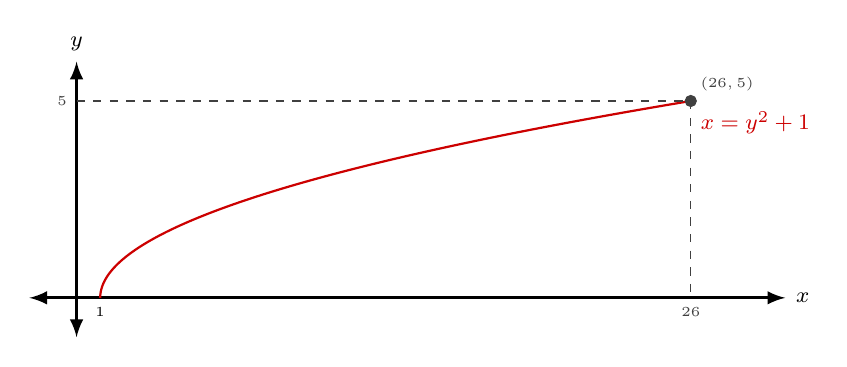
\begin{tikzpicture}[x=0.3cm,y=0.5cm]
            \def\fy{\y*\y+1}

            %axes
            \draw[latex-latex,very thick] (-2,0)--(30,0) node [right] {\footnotesize$x$};
            \draw[latex-latex,very thick] (0,-1)--(0,6) node [above] {\footnotesize$y$};

            %graphs
            \draw[domain=0:5,smooth,samples=120,variable=\y, red!80!black, thick] plot ({\fy},{\y}) node [below right] {\footnotesize$x=y^2+1$};

            %intersection points
            \draw[fill=black,darkgray] (26,5) circle (2pt) node [above right] {\tiny$(26,5)$};
            \draw[darkgray,dashed] (0,5) node[left] {\tiny$5$} -- (26,5) -- (26,0) node[below] {\tiny$26$};
            \node at (1,0) [below] {\tiny$1$};
            \end{tikzpicture}
        \end{center}
        \item Dengan menggunakan turunan implisit pada persamaan grafik \( x = y^2 + 1 \), diperoleh
        \begin{align*}
            \frac{d}{dx}(x) &= \frac{d}{dx}(y^2 + 1) \\
            1 &= 2y \frac{dy}{dx} \\
            \frac{dy}{dx} &= \frac{1}{2y}
        \end{align*}
        Kemudian, substitusi \( y = t = \dfrac{1}{2} \) sehingga didapatkan gradien garis singgung di titik $\left(\dfrac{5}{4}, \dfrac{1}{2}\right)$ adalah 
        \[m=\left.\frac{dy}{dx}\right|_{y=\frac{1}{2}} = \frac{1}{2(\frac{1}{2})} = 1\]
        Dengan demikian, persamaan garis singgung pada titik tersebut adalah
        \begin{align*}
            y - \frac{1}{2} &= 1\left(x - \frac{5}{4}\right) \\
            y &= x - \frac{3}{4}\\
            &\boxed{4x-4y - 3 = 0}
        \end{align*}
      \end{enumerate}
      \item Ilustrasikan terlebih dahulu daerah yang irisannya
        \begin{center}
            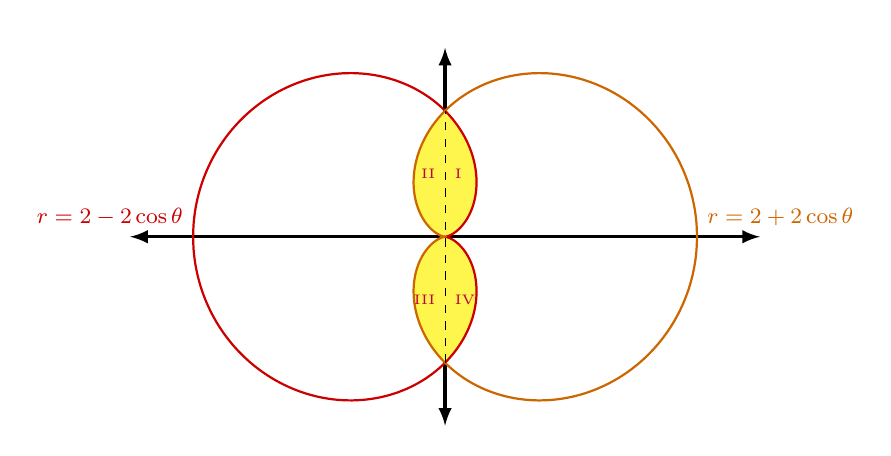
\begin{tikzpicture}[scale=0.8]
            \def\fr{2-2*cos(\o r)}
            \def\gr{2+2*cos(\o r)}
            %axes
            \draw[latex-latex,very thick] (-5,0)--(5,0) node [right] {};
            \draw[latex-latex,very thick] (0,-3)--(0,3) node [above] {};

            %shading
            \fill[domain=0:pi/2,smooth,samples=100,variable=\o, yellow!70] plot ({deg(\o)}:{\fr}) -- plot ({deg(\o+pi/2)}:{2+2*cos((\o+pi/2) r)})--cycle;
            \fill[domain=pi:3*pi/2,smooth,samples=100,variable=\o, yellow!70] plot ({deg(\o)}:{\gr}) -- plot ({deg(\o+pi/2)}:{2-2*cos((\o+pi/2) r)})--cycle;
    
            %graphs
            \draw[domain=-pi:pi,smooth,samples=120,variable=\o, red!80!black, thick] plot ({deg(\o)}:{\fr}) node [above left] {\footnotesize$r=2-2\cos\theta$};
            \draw[domain=2*pi:0,smooth,samples=120,variable=\o, orange!80!black, thick] plot ({deg(\o)}:{\gr}) node [above right] {\footnotesize$r=2+2\cos\theta$};

            
            \draw[dashed] (0,-2) -- (0,2);

            %Area label
            \node at (0,1) [right,purple] {\tiny I};
            \node at (0,1) [left,purple] {\tiny II};
            \node at (0,-1) [right,purple] {\tiny IV};
            \node at (0,-1) [left,purple] {\tiny III};
            \end{tikzpicture}
        \end{center}
        Perhatikan bahwa keempat daerah yang diarsir tersebut memiliki luas yang sama, sehingga total luas daerah yang diarsir adalah empat kali luas salah satu daerah tersebut.
        \begin{align*}
            \text{Area} &= 4 \cdot \frac{1}{2} \int_{0}^{\frac{\pi}{2}} (2 - 2\cos\theta)^2 \, d\theta \\
            &= 2 \int_{0}^{\frac{\pi}{2}} \left( 4 - 8\cos\theta + 4\cos^2\theta \right) \, d\theta \\
            &= 8 \int_{0}^{\frac{\pi}{2}} \left( 1 - 2\cos\theta + \cos^2\theta \right) \, d\theta \\
            &= 8 \int_{0}^{\frac{\pi}{2}} \left( 1 - 2\cos\theta + \frac{1 + \cos(2\theta)}{2} \right) \, d\theta \\
            &= 8 \int_{0}^{\frac{\pi}{2}} \left( \frac{3}{2} - 2\cos\theta + \frac{1}{2}\cos(2\theta) \right) \, d\theta \\
            &= 8 \left[ \frac{3}{2}\theta - 2\sin\theta + \frac{1}{4}\sin(2\theta) \right]_{0}^{\frac{\pi}{2}} \\
            &= 8 \left[ \frac{3}{2}\cdot\frac{\pi}{2} - 2\cdot1 + \frac{1}{4}\cdot0 - \left( \frac{3}{2}\cdot0 - 2\cdot0 + \frac{1}{4}\cdot0 \right) \right] \\
            &= 8 \left[ \frac{3\pi}{4} - 2 \right] = \boxed{6\pi - 16 }
        \end{align*}
      \item Secara umum rumus deret Maclaurin untuk fungsi \( f(x) \) adalah
        \[
            f(x) = \sum_{n=0}^{\infty} \frac{f^{(n)}(0)}{n!} x^n = f(0) + f'(0)x + \frac{f''(0)}{2!}x^2 + \frac{f'''(0)}{3!}x^3 + \cdots
        \]
        Secara berkelanjutan kita tahu bahwa untuk fungsi \( f(x) = e^x\), maka $f^{(n)}(0) = 1$ untuk setiap $n\in\mathbb{N}$, sehingga didapatkan deret Maclaurin untuk fungsi tersebut adalah
        \[
            e^x = \sum_{n=0}^{\infty} \frac{x^n}{n!} = 1 + x + \frac{x^2}{2!} + \frac{x^3}{3!} + \cdots
        \]
        Dengan menggantikan \( x \) dengan \( -x^2 \), maka didapatkan deret Maclaurin untuk fungsi \( f(x) = e^{-x^2} \) adalah
        \[
            e^{-x^2} = \sum_{n=0}^{\infty} \frac{(-x^2)^n}{n!} = 1 - x^2 + \frac{x^4}{2!} - \frac{x^6}{3!} + \frac{x^8}{4!} + \cdots
        \]
        \[
            \boxed{P_5(x) = 1 - x^2 + \frac{x^4}{2}}
        \]
    \end{enumerate}

    \newpage
    \pagestyle{problems}

    \begin{center}
	{\underline{\textbf{\MakeUppercase{Evaluasi Akhir Semester Bersama Genap 2023/2024}}}}
    \end{center}

    \begin{center}
	\begin{tabular}{lcl}
		Mata kuliah/SKS & : & Kalkulus 2 ( SM234201 ) / 3 SKS\\
		Hari, Tanggal & : & Rabu, 26 Juni 2024\\
		Waktu & : & 09.00-10.40 WIB (100 menit)\\
		Sifat & : & Tertutup\\
		Kelas & : & 15-27, 102
	\end{tabular}
    \end{center}
	
    \noindent\rule{\textwidth}{2.pt}
	
    \setlength{\parindent}{5pt}
    \par Diberikan 5 soal, dengan bobot nilai masing-masing soal sama dan boleh dikerjakan tidak berurutan.
    \setlength{\parindent}{5pt}
    \centering{Tuliskan: Nama, NRP, dan Nomor Kelas pada lembar jawaban Anda.}
    \setlength{\parindent}{5pt}
    {\small
    \par \textbf{\MakeUppercase{Dilarang membawa/menggunakan kalkulator dan alat komunikasi}}
    \centering{\textbf{\MakeUppercase{dilarang memberikan/menerima jawaban selama ujian}}}}
    \par \centering{\textbf{"Setiap tindak kecurangan akan mendapat sanksi akademik."}}
	
    \noindent\rule{\textwidth}{2.pt}
	
% SOAL DI SINI YAA
\begin{enumerate}
    \item Dapatkan luas daerah yang dibatasi oleh \( y = x^2 - 4x + 3 \) dan \( y = x + 3 \).

    \item Dapatkan volume benda putar jika daerah yang dibatasi oleh kurva-kurva 
    \( y = \frac{1}{x} \), \( x = 2 \), dan \( y = 2 \) diputar terhadap sumbu-\( x \). 
    Buatlah sketsa daerah tersebut.

    \item Diberikan persamaan parametrik \( x = \cos 2t \), \( y = 3 - 2 \cos 2t \) pada \( 0 \leq t \leq \frac{\pi}{2} \).
    \begin{enumerate}
        \item Dapatkan panjang kurva dari persamaan parametrik.
        \item Buatlah sketsa kurva tersebut.
    \end{enumerate}

    \item Dapatkan luas daerah yang berada di dalam \( r = 2 - 2 \cos \theta \) dan di luar kardioida 
    \( r = 2 + 2 \cos \theta \).

    \item Dapatkan deret Maclaurin untuk fungsi \( f(x) = \ln(1 + x) \).
\end{enumerate}
	
    \fancyfoot{
    \hrulefill\textbf{ Selamat Mengerjakan }\hrulefill

    \begin{center}
	    ``\textit{Jujur adalah kunci kesuksesan}''
    \end{center}}

    \newpage
    \pagestyle{solution}
    {\centering\textbf{SOLUSI}}
    \begin{enumerate}
      \item Titik potong kedua kurva didapatkan dengan menyamakan kedua persamaan tersebut:
        \begin{align*}
            x^2 - 4x + 3 &= x + 3 \\
            x^2 - 5x &= 0 \\
            x(x-5) &= 0 \\
            x = 0 \quad&\vee\quad x = 5
        \end{align*}
        
      
      Daerah yang dibatasi diilustrasikan dibawah ini
      \begin{center}
        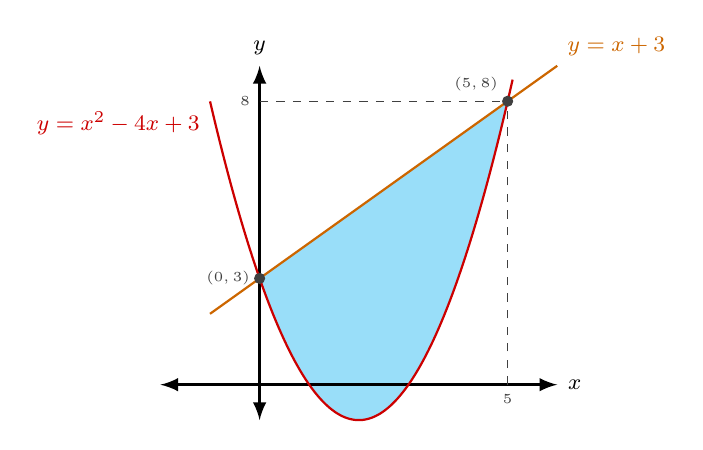
\begin{tikzpicture}[scale=0.9,x=0.7cm,y=0.5cm]
          \def\fx{\x*\x-4*\x+3}
          \def\gx{\x+3}
          %shading
          \fill[domain=0:5,smooth,samples=100,variable=\x, cyan!40] plot ({\x},{\fx})--cycle;
            
          %axes
          \draw[latex-latex,very thick] (-2,0)--(6,0) node [right] {\footnotesize$x$};
          \draw[latex-latex,very thick] (0,-1)--(0,9) node [above] {\footnotesize$y$};
            
          %graphs
          \draw[domain=5.1:-1,smooth,samples=120,variable=\x, red!80!black, thick] plot ({\x},{\fx}) node [below left] {\footnotesize$y=x^2-4x+3$};
          \draw[domain=-1:6,smooth,variable=\x, thick, orange!80!black] plot ({\x},{\gx}) node [above right] {\footnotesize$y=x+3$};
            
          %intersection points
          \draw[fill=black,darkgray] (5,8) circle (2pt) node [above left] {\tiny$(5,8)$};
          \draw[fill=black,darkgray] (0,3) circle (2pt) node [left] {\tiny$(0,3)$};
          \draw[darkgray,dashed] (0,8) node[left] {\tiny$8$} -- (5,8);
          \draw[darkgray,dashed] (5,0) node[below] {\tiny$5$} -- (5,8);
        \end{tikzpicture}
    \end{center}
    Sehingga luas daerah yang diarsir dapat dihitung dengan integral
        \begin{align*}
            \text{Area} &= \int_{0}^{5} (x + 3 - (x^2 - 4x + 3)) \, dx \\
            &= \int_{0}^{5} (5x - x^2) \, dx \\
            &= \left[ \frac{5}{2}x^2 - \frac{1}{3}x^3 \right]_{0}^{5} = \left( \frac{5}{2}(5)^2 - \frac{1}{3}(5)^3 \right) - 0 \\
            &= \frac{125}{2} - \frac{125}{3} = \frac{375 - 250}{6} = \boxed{\frac{125}{6}}
        \end{align*}
      \item Sketsa daerah dapat dilihat di bawah ini
    \begin{center}
        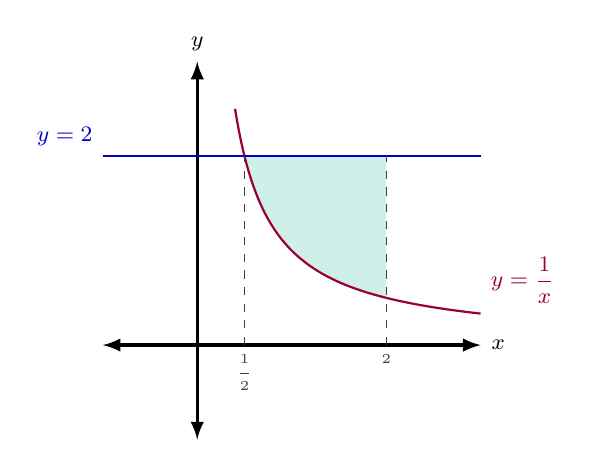
\begin{tikzpicture}[scale=1.2]
        \def\fx{1/\x}
        \def\gx{2}
        %shading
        \fill[domain=0.5:2,smooth,samples=100,variable=\x, Acolor!40] plot ({\x},{\fx})--(2,2)--cycle;

        %axes
        \draw[latex-latex,very thick] (-1,0)--(3,0) node [right] {\footnotesize$x$};
        \draw[latex-latex,very thick] (0,-1)--(0,3) node [above] {\footnotesize$y$};

        %graphs
        \draw[domain=0.4:3,smooth,samples=120,variable=\x, purple!80!black, thick] plot ({\x},{\fx}) node [above right] {\footnotesize$y=\dfrac{1}{x}$};
        \draw[domain=3:-1,smooth,variable=\x, thick, blue!80!black] plot ({\x},{\gx}) node [above left] {\footnotesize$y=2$};

        %intersection points
        \draw[darkgray,dashed] (2,0) node[below] {\tiny$2$} -- (2,2);
        \draw[darkgray,dashed] (0.5,0) node[below] {\tiny$\dfrac{1}{2}$} -- (0.5,2);
        \end{tikzpicture}
      \end{center}
      Selanjutnya daerah yang diarsir diputar terhadap sumbu-\( x \), sehingga akan digunakan metode cakram untuk menghitung volume benda putar.
      \begin{center}
        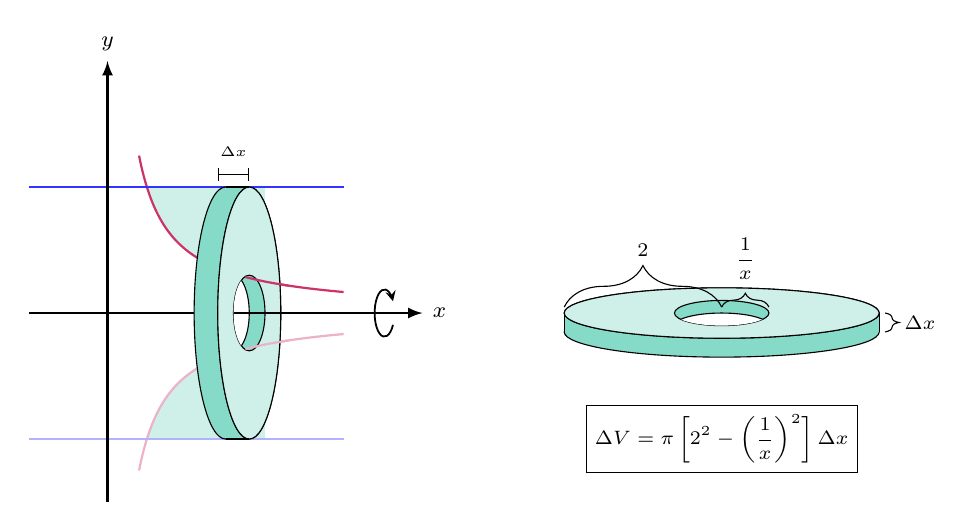
\begin{tikzpicture}[>=latex,x=1cm,y=0.8cm]
            \def\fx{1/\x}
            \def\gx{2}

            \fill[domain=0.5:2,smooth,samples=100,variable=\x, Acolor!40] plot ({\x},{\fx})--(2,2)--cycle;
            \fill[domain=0.5:2,smooth,samples=100,variable=\x, Acolor!40] plot ({\x},{-\fx})--(2,-2)--cycle;

            \draw[domain=0.4:3,smooth,samples=120,variable=\x, purple!80, thick] plot ({\x},{\fx});
            \draw[domain=0.4:3,smooth,samples=120,variable=\x, purple!30, thick] plot ({\x},{-\fx});
            
            \draw[domain=3:-1,smooth,variable=\x, thick, blue!80] plot ({\x},{\gx});
            \draw[domain=3:-1,smooth,variable=\x, thick, blue!30] plot ({\x},{-\gx});

            \draw[fill=Acolor] (1.5,0) circle [y radius =2 , x radius =.4];
            \fill[Acolor] (1.8,2) rectangle (1.5,-2);
            \draw[fill=Acolor!40] (1.8,0) circle [y radius =2 , x radius =.4];
            \draw[fill=Acolor!40] (1.8,0) circle [y radius =2 , x radius =.4];
            \draw[fill=Acolor] (1.8,0) circle [y radius =.6 , x radius =.2];
            \draw[thin] (1.5,2) -- (1.8,2);
            \draw[thin] (1.5,-2) -- (1.8,-2);
            \begin{scope}
                \clip (1.8,0) circle [y radius =.6 , x radius =.2];
                \draw[fill=white] (1.6,0) circle [y radius =.6 , x radius =.2];
            \end{scope}

            \draw[->, thick] (1.6,0) -- (4,0) node[right] {\footnotesize $x$};
            \node at (3.5,0) {\AxisRotator};
            \draw[thick] (-1,0) -- (1.1,0);
            \draw[->, thick] (0,-3) -- (0,4) node[above]{\footnotesize $y$};

            \draw[domain=1.75:2.3,smooth,samples=120,variable=\x, purple!80, thick] plot ({\x},{\fx});
            \draw[domain=1.75:2.3,smooth,samples=120,variable=\x, purple!30, thick] plot ({\x},{-\fx});

            \draw[|-|] (1.4,2.2) -- (1.8,2.2) node[midway,above,yshift=0.1cm] {\tiny $\Delta x$};

            \begin{scope}[xshift=6cm,font=\scriptsize]
                \draw[fill=Acolor] (1.8,-0.3) circle [x radius =2 , y radius =.4];
                \fill[Acolor] (-0.2,0) rectangle (3.8,-0.3);
                \draw[fill=Acolor!40] (1.8,0) circle [x radius =2 , y radius =.4];
                \draw[fill=Acolor!40] (1.8,0) circle [x radius =2 , y radius =.4];
                \draw[fill=Acolor] (1.8,0) circle [x radius =.6 , y radius =.2];
                \begin{scope}
                    \clip (1.8,0) circle [x radius =.6 , y radius =.2];
                    \draw[fill=white] (1.8,-0.2) circle [x radius =.6 , y radius =.2];
                \end{scope}
                \draw[thin] (-0.2,0) -- (-0.2,-0.3);
                \draw[thin] (3.8,0) -- (3.8,-0.3);

                \draw [decorate,decoration={brace,mirror,raise=0.5ex,amplitude=5pt}] (2.4,0) -- (1.8,0) node[midway,above,yshift=0.3cm]{$\dfrac{1}{x}$};
                \draw [decorate,decoration={brace,mirror,raise=0.5ex,amplitude=15pt}] (1.8,0) -- (-0.2,0) node[midway,above,yshift=0.6cm]{$2$};
                \draw [decorate,decoration={brace,mirror,raise=0.5ex,amplitude=5pt}] (3.8,-.3) -- (3.8,0) node[midway,right,xshift=0.2cm]{$\Delta x$};

                \node at (1.8,-2) {$\displaystyle\boxed{\Delta V=\pi\left[2^2-\left(\dfrac{1}{x}\right)^2\right] \Delta x}$};
            \end{scope}
        \end{tikzpicture}
    \end{center}
        Maka volume benda putar yang dihasilkan jika dilihat dari salah satu potongan silinder diatas adalah
        \begin{align*}
            V &= \pi \int_{\frac{1}{2}}^{2} \left[ 2^2 - \left( \frac{1}{x} \right)^2 \right] \, dx \\
            &= \pi \int_{\frac{1}{2}}^{2} \left( 4 - \frac{1}{x^2} \right) \, dx \\
            &= \pi \left[ 4x + \frac{1}{x} \right]_{\frac{1}{2}}^{2} = \pi\left[ 4(2) + \frac{1}{2} - (2 + 2) \right] = \boxed{\frac{9}{2}\pi}
        \end{align*}

      \item 
      \begin{enumerate}
        \item \underline{Cara pertama:} Gunakan integral panjang kurva parametrik yaitu
        \[
        S = \int_{a}^{b} \sqrt{\left(\frac{dx}{dt}\right)^2 + \left(\frac{dy}{dt}\right)^2} \, dt
        \]
        Maka, kita perlu menghitung turunan \( x \) dan \( y \) terhadap \( t \):
        \begin{align*}
            \frac{dx}{dt} &= -2\sin 2t \\
            \frac{dy}{dt} &= -4\sin 2t
        \end{align*}
        Sehingga panjang kurva dapat dihitung sebagai berikut:
        \begin{align*}
            S &= \int_{0}^{\frac{\pi}{2}} \sqrt{\left(-2\sin 2t\right)^2 + \left(-4\sin 2t\right)^2} \, dt \\
            &= \int_{0}^{\frac{\pi}{2}} \sqrt{20\sin^2 2t} \, dt \\
            &= 2\sqrt{5} \int_{0}^{\frac{\pi}{2}} \sin 2t \, dt \\
            &= 2\sqrt{5} \left[ -\frac{1}{2}\cos 2t \right]_{0}^{\frac{\pi}{2}} \\
            &= 2\sqrt{5} \left[ -\frac{1}{2}\left(-2\right) \right] = 2\sqrt{5} \cdot 1 = \boxed{2\sqrt{5}}
        \end{align*}
        \underline{Cara kedua:} Substitusi \( x = \cos 2t \) pada persamaan $y = 3 - 2\cos 2t$. Kemudian untuk domainnya kita bisa mencari nilai maksimum dan minimum dari \( x \) terhadap domain $t$, yaitu
        \begin{align*}
            t=0 &\Rightarrow x = \cos 0 = 1 \\
            t=\frac{\pi}{2} &\Rightarrow x = \cos \pi = -1
        \end{align*}
        Sehingga didapatkan persamaan kartesiusnya
        \begin{align*}
            y &= 3 - 2x, \quad -1 \leq x \leq 1
        \end{align*}
        Karena \( y \) adalah fungsi linear garis lurus, maka panjang kurva dapat dihitung dengan rumus jarak antara dua titik ujungnya yaitu $(-1, 5)$ dan $(1, 1)$
        \begin{align*}
            S &= \sqrt{(x_2 - x_1)^2 + (y_2 - y_1)^2} \\
            &= \sqrt{(1 - (-1))^2 + (1 - 5)^2} \\
            &= \sqrt{(2)^2 + (-4)^2} = \sqrt{4 + 16} = \sqrt{20} = \boxed{2\sqrt{5}}
        \end{align*}
        \item Menggunakan \underline{cara kedua} pada poin (a), kita sudah mendapatkan persamaan kartesiusnya dengan domainnya juga. Sketsa kurva tersebut adalah sebagai berikut:
        \begin{center}
            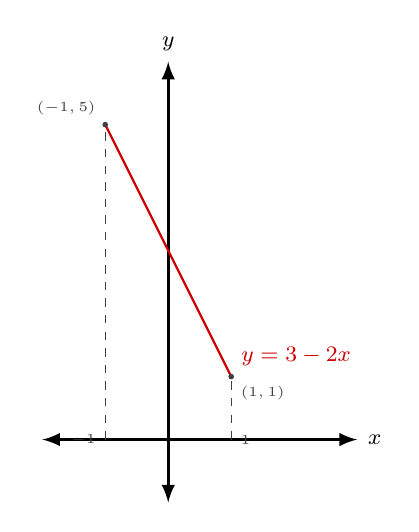
\begin{tikzpicture}[scale=0.8]
            \def\fx{3-2*\x}
            %axes
            \draw[latex-latex,very thick] (-2,0)--(3,0) node [right] {\footnotesize$x$};
            \draw[latex-latex,very thick] (0,-1)--(0,6) node [above] {\footnotesize$y$};

            %graphs
            \draw[domain=-1:1,smooth,samples=120,variable=\x, red!80!black, thick] plot ({\x},{\fx}) node [above right] {\footnotesize$y=3-2x$};

            %intersection points
            \draw[fill=black,darkgray] (-1,5) circle (1pt) node [above left] {\tiny$(-1,5)$};
            \draw[fill=black,darkgray] (1,1) circle (1pt) node [below right] {\tiny$(1,1)$};
            \draw[darkgray,dashed] (-1,0) node[left] {\tiny$-1$} -- (-1,5);
            \draw[darkgray,dashed] (1,0) node[right] {\tiny$1$} -- (1,1);
            \end{tikzpicture}
        \end{center}
      \end{enumerate}
      \item Sketsa daerah yang diarsir dapat dilihat di bawah ini
    \begin{center}
        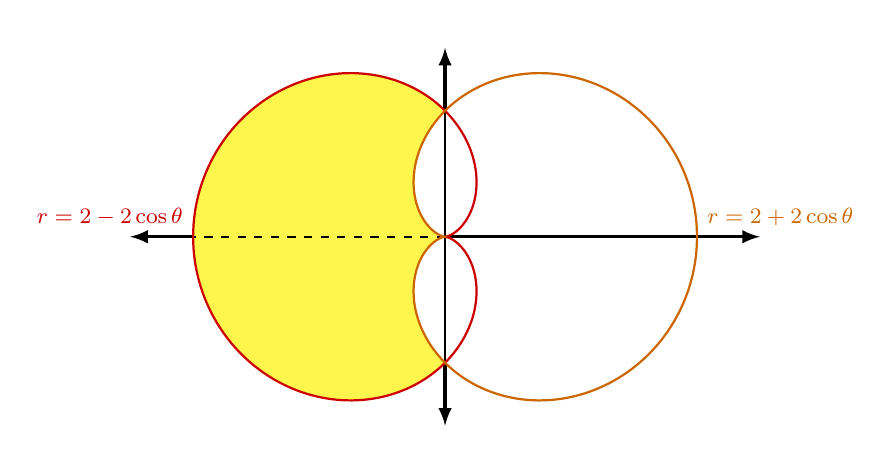
\begin{tikzpicture}[scale=0.8]
        \def\fr{2-2*cos(\o r)}
        \def\gr{2+2*cos(\o r)}
        %axes
        \draw[latex-latex,very thick] (-5,0)--(5,0) node [right] {};
        \draw[latex-latex,very thick] (0,-3)--(0,3) node [above] {};

        %shading
        \begin{scope}
            \fill[domain=0:2*pi,smooth,samples=100,variable=\o, yellow!70] plot ({deg(\o)}:{\fr});
            \fill[domain=-pi/2:pi/2,smooth,samples=100,variable=\o, white] plot ({deg(\o)}:{\fr}) --cycle;
            \fill[domain=pi/2:3*pi/2,variable=\o,smooth,samples=100,white] plot ({deg(\o)}:{\gr})--cycle;
        \end{scope}
       
        \draw[thick] (0,2) -- (0,-2);
        \draw[thick,dashed] (0,0) -- (-4,0);

        %graphs
        \draw[domain=-pi:pi,smooth,samples=120,variable=\o, red!80!black, thick] plot ({deg(\o)}:{\fr}) node [above left] {\footnotesize$r=2-2\cos\theta$};
        \draw[domain=2*pi:0,smooth,samples=120,variable=\o, orange!80!black, thick] plot ({deg(\o)}:{\gr}) node [above right] {\footnotesize$r=2+2\cos\theta$};
        \end{tikzpicture}
    \end{center}
    Perhatikan untuk daerah yang diarsir bisa diperoleh dengan menghitung luas daerah $r=2-2\cos\theta$ dan mengurangkan luas daerah $r=2+2\cos\theta$ dari $\pi$ sampai $3\pi/2$.
    \begin{align*}
        \text{Area} &= \frac{1}{2} \int_{\pi}^{\frac{3\pi}{2}} \left( (2 - 2\cos\theta)^2 - (2 + 2\cos\theta)^2 \right) \, d\theta \\
        &= \int_{\pi/2}^{\pi} \left( 4 - 8\cos\theta + 4\cos^2\theta \right) - \left( 4 + 8\cos\theta + 4\cos^2\theta \right) \, d\theta \\
        &= -16\int_{\pi/2}^{\pi} \cos\theta \, d\theta = -16 \left[ \sin\theta \right]_{\pi/2}^{\pi} = -16 \left( 0 - 1 \right) = 16 
    \end{align*}
      \item Diketahui bahwa untuk setiap fungsi \( f(x) \) yang dapat diturunkan, deret Maclaurin dapat dituliskan sebagai
        \[
            f(x) = \sum_{n=0}^{\infty} \frac{f^{(n)}(0)}{n!} x^n
        \]
        \underline{Cara pertama:} Untuk fungsi \( f(x) = \ln(1+x) \), kita perlu menghitung turunan-turunan dari \( f(x) \) pada \( x = 0 \):
        \begin{align*}
            f(0) &= \ln(1+0) = 0,\\
            f'(x) &= \frac{1}{1+x} \Rightarrow f'(0) = 1,\\
            f''(x) &= -\frac{1}{(1+x)^2} \Rightarrow f''(0) = -1,\\
            f'''(x) &= \frac{2}{(1+x)^3} \Rightarrow f'''(0) = 2,\\
            f^{(4)}(x) &= -\frac{6}{(1+x)^4} \Rightarrow f^{(4)}(0) = -6,\\
            &\vdots
        \end{align*}
        Dengan demikian, deret Maclaurin untuk fungsi tersebut adalah
        \[
            f(x) = 0  + 1\cdot x + (-1)\frac{x^2}{2!} + (2)\frac{x^3}{3!} + (-6)\frac{x^4}{4!} + \cdots = \boxed{x - \frac{x^2}{2} + \frac{x^3}{3} - \frac{x^4}{4} + \cdots}
        \]
        \underline{Cara kedua:} ingat bahwa untuk \( |x| < 1 \), kita memiliki deret geometri 
        \[
            \frac{1}{1-x} = \sum_{n=0}^{\infty} x^n =1 + x + x^2 + x^3 + \cdots
        \]
        Kemudian ganti \( x \) dengan \( -x \) sehingga didapatkan
        \[
            \frac{1}{1+x} =1 - x + x^2 - x^3 + \cdots
        \]
        Dengan mengintegrasikan kedua sisi, kita mendapatkan
        \begin{align*}
            \int \frac{1}{1+x} \, dx &= \int (1 - x + x^2 - x^3 + \cdots) \, dx \\
            \ln(1+x) &= x - \frac{x^2}{2} + \frac{x^3}{3} - \frac{x^4}{4} + \cdots + C
        \end{align*}
        Dengan \( C = 0 \) karena \( \ln(1+0) = 0 \), maka didapatkan deret Maclaurin untuk fungsi tersebut adalah
        \[
            f(x) = x - \frac{x^2}{2} + \frac{x^3}{3} - \frac{x^4}{4} + \cdots= \boxed{\sum_{n=1}^{\infty} (-1)^{n-1} \frac{x^n}{n}}
        \]

    \end{enumerate}

    \newpage
    \pagestyle{problems}
    
    \begin{center}
	{\underline{\textbf{\MakeUppercase{Evaluasi Akhir Semester Bersama Genap 2023/2024}}}}
    \end{center}

    \begin{center}
	\begin{tabular}{lcl}
		Mata kuliah/SKS & : & Kalkulus 2 ( SM234201 ) / 3 SKS\\
		Hari, Tanggal & : & Rabu, 26 Juni 2024\\
		Waktu & : & 11.00-12.40 WIB (100 menit)\\
		Sifat & : & Tertutup\\
		Kelas & : & 31-38, 104
	\end{tabular}
    \end{center}
	
    \noindent\rule{\textwidth}{2.pt}
	
    \setlength{\parindent}{5pt}
    \par Diberikan 5 soal, dengan bobot nilai masing-masing soal sama dan boleh dikerjakan tidak berurutan.
    \setlength{\parindent}{5pt}
    \centering{Tuliskan: Nama, NRP, dan Nomor Kelas pada lembar jawaban Anda.}
    \setlength{\parindent}{5pt}
    {\small
    \par \textbf{\MakeUppercase{Dilarang membawa/menggunakan kalkulator dan alat komunikasi}}
    \centering{\textbf{\MakeUppercase{dilarang memberikan/menerima jawaban selama ujian}}}}
    \par \centering{\textbf{"Setiap tindak kecurangan akan mendapat sanksi akademik."}}
	
    \noindent\rule{\textwidth}{2.pt}
	
% SOAL DI SINI YAA
\begin{enumerate}
    \item Dapatkan luas daerah yang dibatasi oleh \( y = -x^2 + 2x + 3 \) dan \( y + 2x = 3 \).

    \item Gambarkan daerah yang dibatasi oleh kurva-kurva \( y = 2x - x^2 \) dan \( y = x^2 - 2x \). 
    Menggunakan Dalil Guldin I, dapatkan volume benda padat jika daerah tersebut diputar terhadap garis \( y = 2 \).

    \item Diberikan persamaan parametrik \( x = \sin t \), \( y = 1 + 2\sin t \), 
    \( 0 \leq t \leq \frac{\pi}{2} \).
    \begin{enumerate}
        \item Dapatkan panjang kurva dari persamaan parametrik.
        \item Buatlah sketsa kurva tersebut.
    \end{enumerate}

    \item Dapatkan luas daerah yang berada di dalam lingkaran \( r = 4\sin \theta \) 
    dan di luar lingkaran \( r = 4\cos \theta \).

    \item Dapatkan deret Taylor untuk fungsi \( f(x) = \dfrac{1}{5 - 4x} \) di sekitar \( x = 1 \).
\end{enumerate}
	
    \fancyfoot{
    \hrulefill\textbf{ Selamat Mengerjakan }\hrulefill

    \begin{center}
	    ``\textit{Jujur adalah kunci kesuksesan}''
    \end{center}}

    \newpage
    \pagestyle{solution}
    {\centering\textbf{SOLUSI}}

    \begin{enumerate}
      \item Titik potong kedua kurva didapatkan dengan menyamakan kedua persamaan tersebut:
        \begin{align*}
            -x^2 + 2x + 3 &= -2x + 3 \\
            -x^2 + 4x &= 0 \\
            x(x-4) &= 0 \\
            x = 0 \quad&\vee\quad x = 4
        \end{align*}
        Daerah yang dibatasi diilustrasikan dibawah ini
        \begin{center}
            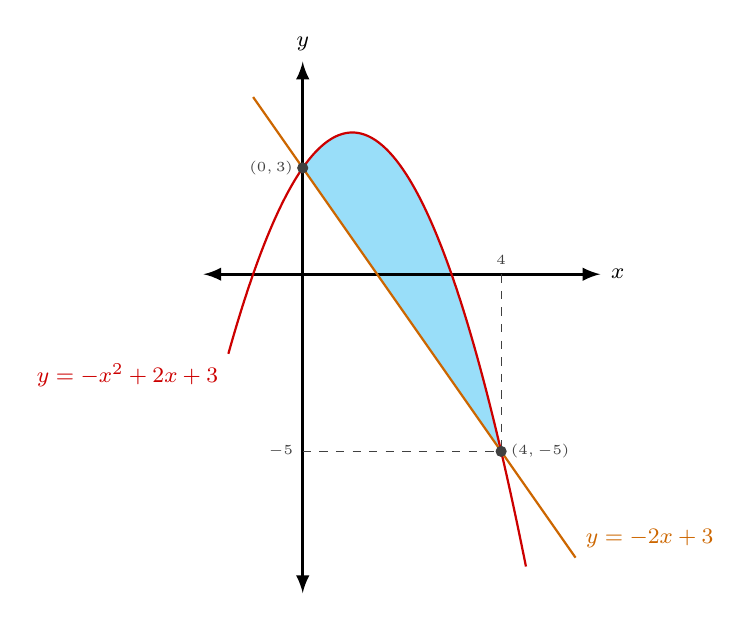
\begin{tikzpicture}[scale=0.9,x=0.7cm,y=0.5cm]
                \def\fx{-\x*\x+2*\x+3}
                \def\gx{-2*\x+3}
                %shading
                \fill[domain=0:4,smooth,samples=100,variable=\x, cyan!40] plot ({\x},{\fx})--cycle;
                %axes
                \draw[latex-latex,very thick] (-2,0)--(6,0) node [right] {\footnotesize$x$};
                \draw[latex-latex,very thick] (0,-9)--(0,6) node [above] {\footnotesize$y$};
                %graphs
                \draw[domain=4.5:-1.5,smooth,samples=120,variable=\x, red!80!black, thick] plot ({\x},{\fx}) node [below left] {\footnotesize$y=-x^2+2x+3$};
                \draw[domain=-1:5.5,smooth,variable=\x, thick, orange!80!black] plot ({\x},{\gx}) node [above right] {\footnotesize$y=-2x+3$};
                %intersection points
                \draw[fill=black,darkgray] (4,-5) circle (2pt) node [right] {\tiny$(4,-5)$};
                \draw[fill=black,darkgray] (0,3) circle (2pt) node [left] {\tiny$(0,3)$};
                \draw[darkgray,dashed] (4,0) node[above] {\tiny$4$} -- (4,-5);
                \draw[darkgray,dashed] (0,-5) node[left] {\tiny$-5$} -- (4,-5);
            \end{tikzpicture}
        \end{center}
        Sehingga luas daerah yang diarsir dapat dihitung dengan integral berikut
        \begin{align*}
            \text{Area} &= \int_{0}^{4} -x^2 + 2x + 3 - (-2x + 3) \, dx \\
            &= \int_{0}^{4} -x^2 + 4x \, dx \\
            &= \left[ -\frac{1}{3}x^3 + 2x^2 \right]_{0}^{4} = \left( -\frac{1}{3}(4)^3 + 2(4)^2 \right) - 0 \\
            &= -\frac{64}{3} + 32 = \boxed{\frac{32}{3}}
        \end{align*}
        \item Titik potong kedua kurva didapatkan dengan menyamakan kedua persamaan tersebut:
        \begin{align*}
            2x - x^2 &= x^2 - 2x \\
            4x &= 2x^2 \\
            0 &= 2x^2 - 4x \\
            0 &= 2x(x-2) \\
            x = 0 \quad&\vee\quad x = 2
        \end{align*}
        Daerah yang dibatasi diilustrasikan dibawah ini
        \begin{center}
            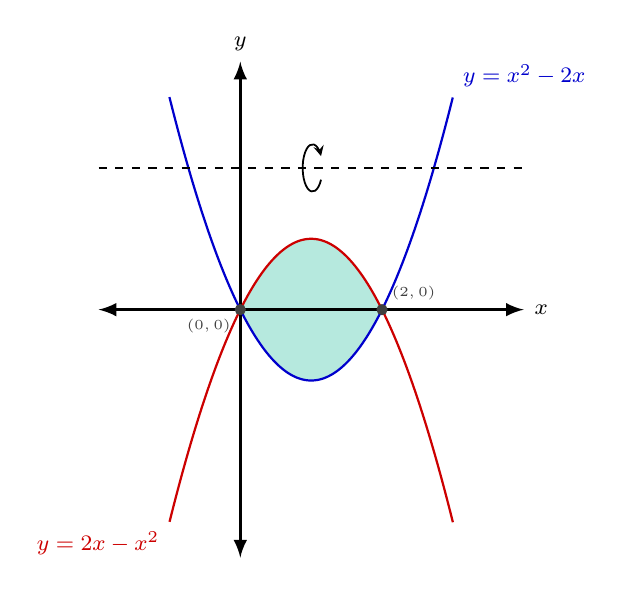
\begin{tikzpicture}[scale=0.9]
                \def\fx{2*\x-\x*\x}
                \def\gx{-2*\x+\x*\x}
                %shading
                \fill[domain=0:2,smooth,samples=100,variable=\x, Acolor!60] plot ({\x},{\fx})--plot ({2-\x},{\gx})--cycle;
                %axes
                \draw[latex-latex,very thick] (-2,0)--(4,0) node [right] {\footnotesize$x$};
                \draw[latex-latex,very thick] (0,-3.5)--(0,3.5) node [above] {\footnotesize$y$};
                %graphs
                \draw[domain=3:-1,smooth,samples=120,variable=\x, red!80!black, thick] plot ({\x},{\fx}) node [below left] {\footnotesize$y=2x-x^2$};
                \draw[domain=-1:3,smooth,samples=120,variable=\x, thick, blue!80!black] plot ({\x},{\gx}) node [above right] {\footnotesize$y=x^2-2x$};
                %intersection points
                \draw[fill=black,darkgray] (2,0) circle (2pt) node [above right] {\tiny$(2,0)$};
                \draw[fill=black,darkgray] (0,0) circle (2pt) node [below left] {\tiny$(0,0)$};

                %Rotation axis
                \draw[thick,dashed] (-2,2) -- (4,2) node [midway] {\AxisRotator};
            \end{tikzpicture}
        \end{center}
        Karena diputar terhadap garis \( y = 2 \), maka kita perlu menghitung jarak titik berat dari garis tersebut yang dimana komponen yang dibutuhkan hanyalah \(\bar{y}\).\footnote{Ilustrasi pada gambar sebenarnya cukup menunjukkan bahwa daerah tersebut simetris terhadap sumbu-$x$, sehingga dapat ditarik kesimpulan \(\bar{y} = 0\).}
        \begin{align*}
            M &= \int_{0}^{2} (2x - x^2)-(x^2-2x) \, dx = \int_{0}^{2} (4x - 2x^2) \, dx \\
            &= \left[ 2x^2 - \frac{2}{3}x^3 \right]_{0}^{2} = \left( 2(2)^2 - \frac{2}{3}(2)^3 \right) - 0 = 8 - \frac{16}{3} = \frac{24-16}{3} = \frac{8}{3}\\
            M_x &= \frac{1}{2}\int_{0}^{2} \left( 2x-x^2\right)^2 - \left( x^2-2x \right)^2 \, dx = \int_{0}^{2} \left( 2x - x^2 + x^2 - 2x \right)\left( 2x-x^2-x^2+2x\right) \, dx \\
            &= \int_{0}^{2} (0)(4x-2x^2) \, dx = 0\\
            \bar{y} &= \frac{M_x}{M} = \frac{0}{\frac{8}{3}} = 0
        \end{align*}
        Ingat rumus Dalil Guldin I untuk volume benda putar yaitu
        \[
            V = 2\pi L \Delta\bar{y}
        \]
        dengan \( \Delta\bar{y} \) adalah jarak antara garis rotasi dengan titik berat daerah yang diarsir yaitu \( \Delta\bar{y} = |2 - \bar{y}| = 2 - 0 = 2 \). $L$ adalah luas daerah yang diarsir yang sudah kita hitung sebelumnya yaitu \( L = M = \frac{8}{3} \).
        Maka volume benda putar yang dihasilkan adalah
        \begin{align*}
            V &= 2\pi(2)\left(\frac{8}{3}\right) = \boxed{\frac{32\pi}{3}}
        \end{align*}
        \item \begin{enumerate}
            \item Turunkan \( x \) dan \( y \) terhadap \( t \):
            \begin{align*}
                \frac{dx}{dt} &= \cos t \\
                \frac{dy}{dt} &= 2\cos t
            \end{align*}
            Maka panjang kurva dapat dihitung dengan rumus integral panjang kurva parametrik yaitu
            \[
                S = \int_{a}^{b} \sqrt{\left(\frac{dx}{dt}\right)^2 + \left(\frac{dy}{dt}\right)^2} \, dt
            \]
            Sehingga panjang kurva dari \( t = 0 \) sampai \( t = \frac{\pi}{2} \) adalah
            \begin{align*}
                S &= \int_{0}^{\frac{\pi}{2}} \sqrt{\left(\cos t\right)^2 + \left(2\cos t\right)^2} \, dt \\
                &= \int_{0}^{\frac{\pi}{2}} \sqrt{5\cos^2 t} \, dt \\
                &= \sqrt{5} \int_{0}^{\frac{\pi}{2}} |\cos t| \, dt = \sqrt{5} \left[ \sin t \right]_{0}^{\frac{\pi}{2}} = \sqrt{5}(1 - 0) = \boxed{\sqrt{5}}
            \end{align*}
            \item Dengan melakukan substitusi \( x = \sin t \), maka didapatkan
            \begin{align*}
                y &= 1+2x,\quad 1 \leq x \leq 3 \\
            \end{align*}
            Sehingga sketsa kurva tersebut adalah sebagai berikut:
            \begin{center}
                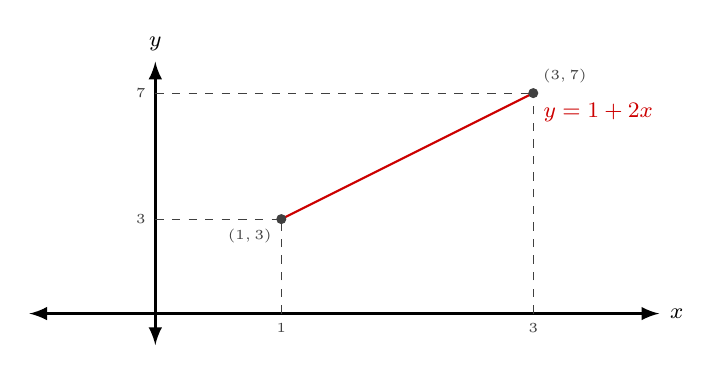
\begin{tikzpicture}[scale=0.8,y=0.5cm,x=2cm]
                %axes
                \draw[latex-latex,very thick] (-1,0)--(4,0) node [right] {\footnotesize$x$};
                \draw[latex-latex,very thick] (0,-1)--(0,8) node [above] {\footnotesize$y$};

                %graphs
                \draw[domain=1:3,smooth,samples=120,variable=\x, red!80!black, thick] plot ({\x},{1+2*\x}) node [below right] {\footnotesize$y=1+2x$};

                %intersection points
                \draw[fill=black,darkgray] (1,3) circle (2pt) node [below left] {\tiny$(1,3)$};
                \draw[fill=black,darkgray] (3,7) circle (2pt) node [above right] {\tiny$(3,7)$};
                \draw[darkgray,dashed] (1,0) node[below] {\tiny$1$} -- (1,3);
                \draw[darkgray,dashed] (3,0) node[below] {\tiny$3$} -- (3,7);
                \draw[darkgray,dashed] (0,3) node[left] {\tiny$3$} -- (1,3);
                \draw[darkgray,dashed] (0,7) node[left] {\tiny$7$} -- (3,7);
                \end{tikzpicture}
            \end{center}
        \end{enumerate}
        \item Titik potong kedua kurva polar didapatkan dengan menyamakan kedua persamaan tersebut:
        \begin{align*}
            4\sin\theta &= 4\cos\theta \\
            \tan\theta &= 1 \\
            \theta &= \frac{\pi}{4}
        \end{align*}
        Sketsa daerah yang diarsir dapat dilihat di bawah ini
        \begin{center}
            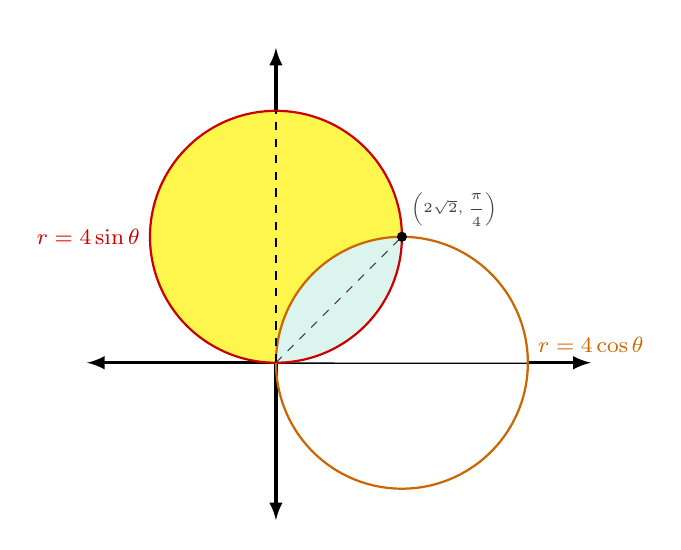
\begin{tikzpicture}[scale=0.8]
            \def\fr{4*sin(\o r)}
            \def\gr{4*cos(\o r)}
            %axes
            \draw[latex-latex,very thick] (-3,0)--(5,0) node [right] {};
            \draw[latex-latex,very thick] (0,-2.5)--(0,5) node [above] {};

            %shading
            \begin{scope}
                \fill[domain=0:pi,smooth,samples=100,variable=\o, yellow!70] plot ({deg(\o)}:{\fr});
                \fill[domain=pi:3*pi/2,variable=\o,smooth,samples=100,white] plot ({deg(\o)}:{\gr})--cycle;
            \end{scope}
            \begin{scope}
                \clip[domain=0:pi/2,variable=\o] plot ({deg(\o)}:{\gr});
                \fill[domain=0:pi/2,smooth,samples=100,variable=\o, Acolor!30] plot ({deg(\o)}:{\fr});
            \end{scope}

            %graphs
            \draw[domain=3*pi/4:7*pi/4,smooth,samples=120,variable=\o, red!80!black, thick] plot ({deg(\o)}:{\fr}) node [left] {\footnotesize$r=4\sin\theta$};
            \draw[domain=2*pi:0,smooth,samples=120,variable=\o, orange!80!black, thick] plot ({deg(\o)}:{\gr}) node [above right] {\footnotesize$r=4\cos\theta$};

            \draw[thick, dashed] (0,0) -- (0,4);
            \draw[darkgray, dashed] (0:0) -- ({deg(pi/4)}:{2*sqrt(2)}) node[above right] {\tiny$\left(2\sqrt{2}, \dfrac{\pi}{4}\right)$};
            \draw[fill=black] ({deg(pi/4)}:{2*sqrt(2)}) circle (2pt);
            \end{tikzpicture}
        \end{center}
        Luas daerah yang dimaksud pada soal adalah 
        \[
        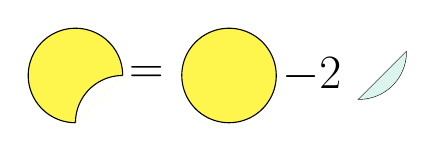
\begin{tikzpicture}[scale=0.3]
            \def\fr{4*sin(\o r)}
            \def\gr{4*cos(\o r)}
            \draw[domain=0:pi,smooth,samples=100,variable=\o, fill=yellow!70] plot ({deg(\o)}:{\fr});

            \begin{scope}[xshift=3.5cm]
                \node at (0,2) {\LARGE$-2$};
            \end{scope}
            \begin{scope}[xshift=5.5cm,yshift=1cm]
                \draw[domain=0:pi/4,smooth,samples=100,variable=\o] plot ({deg(\o)}:{\fr})--cycle;
                \fill[domain=0:pi/4,smooth,samples=100,variable=\o, Acolor!30] plot ({deg(\o)}:{\fr})--cycle;
            \end{scope}

            \begin{scope}[xshift=-3.5cm]
                \node at (0,2) {\LARGE$=$};
            \end{scope}

            \begin{scope}[xshift=-6.5cm]
                \draw[domain=pi/4:pi,smooth,samples=100,variable=\o, fill=yellow!70] plot ({deg(\o)}:{\fr});
                \draw[domain=pi/4:pi/2,smooth,samples=100,variable=\o, fill=white] plot ({deg(\o)}:{\gr});
            \end{scope}
        \end{tikzpicture}
        \]
        Sehingga perhitungan integral yang benar adalah
        \begin{align*}
            \text{Area} &= 4\pi - 2\left[\frac{1}{2}\int_{0}^{\frac{\pi}{4}} 4\sin^2\theta \, d\theta\right]\\
            &= 4\pi - 2\left[\int_{0}^{\frac{\pi}{4}} (1-\cos 2\theta) \, d\theta\right]\\
            &= 4\pi - 2\left[\theta - \frac{1}{2}\sin 2\theta\right]_{0}^{\frac{\pi}{4}}\\
            &= 4\pi - 2\left[\frac{\pi}{4} - \frac{1}{2}\sin \frac{\pi}{2}\right]\\
            &= 4\pi - 2\left[\frac{\pi}{4} - \frac{1}{2}\right]\\
            &= 4\pi - \frac{\pi}{2} + 1 = \boxed{\frac{7\pi}{2} + 1}
        \end{align*}
        \item Diketahui bahwa untuk setiap fungsi \( f(x) \) yang dapat diturunkan, deret Taylor disekitar \( x = a \) dapat dituliskan sebagai
        \[
            f(x) = \sum_{n=0}^{\infty} \frac{f^{(n)}(a)}{n!} (x-a)^n
        \]
        \underline{Cara pertama:} Hitung turunan-turunan dari \( f(x) = \dfrac{1}{5-4x} \) pada \( x = 1 \):
        \begin{align*}
            f(1) &= \frac{1}{5-4\cdot 1} = \frac{1}{1} = 1,\\
            f'(x) &= \frac{4}{(5-4x)^2} \Rightarrow f'(1) = 4,\\
            f''(x) &= -\frac{32}{(5-4x)^3} \Rightarrow f''(1) = -32,\\
            f'''(x) &= \frac{384}{(5-4x)^4} \Rightarrow f'''(1) = 384,\\
            &\vdots
        \end{align*}
        Dengan demikian, deret Taylor untuk fungsi tersebut adalah
        \begin{align*}
            f(x) &= 1 + 4(x-1) - \frac{32}{2!}(x-1)^2 + \frac{384}{3!}(x-1)^3 + \cdots \\
            &= 1 + 4(x-1) - 16(x-1)^2 + 64(x-1)^3 + \cdots \\
            &= \boxed{\sum_{n=0}^{\infty} (-1)^{n-1} 4^{n-1} (x-1)^n}
        \end{align*}
        \underline{Cara kedua:} Perhatikan bahwa kita dapat menulis fungsi tersebut sebagai
        \[
            f(x) = \frac{1}{1+(4-4x)} = \frac{1}{1+4(1-x)} 
        \]
        Dengan jari-jari konvergensi \( |x-1| < \frac{1}{4} \), dapat kita substitusikan $y=x-1$ sehingga didapatkan
        \[
            f(x) = \frac{1}{1-(-4y)} = \frac{1}{1+4y}
        \]
        Terakhir menggunakan deret geometri dapat diperoleh
        \[
            f(x) = \frac{1}{1+4y}=\sum_{n=0}^{\infty} (-4y)^n = \boxed{\sum_{n=0}^{\infty} (-1)^{n-1} 4^{n-1} (x-1)^n}
        \]
    \end{enumerate}

    \newpage
    \pagestyle{problems}
    
    \begin{center}
	{\underline{\textbf{\MakeUppercase{Evaluasi Akhir Semester Bersama Genap 2023/2024}}}}
    \end{center}

    \begin{center}
	\begin{tabular}{lcl}
		Mata kuliah/SKS & : & Kalkulus 2 ( SM234201 ) / 3 SKS\\
		Hari, Tanggal & : & Rabu, 26 Juni 2024\\
		Waktu & : & 13.30-15.10 WIB (100 menit)\\
		Sifat & : & Tertutup\\
		Kelas & : & 40-63
	\end{tabular}
    \end{center}
	
    \noindent\rule{\textwidth}{2.pt}
	
    \setlength{\parindent}{5pt}
    \par Diberikan 5 soal, dengan bobot nilai masing-masing soal sama dan boleh dikerjakan tidak berurutan.
    \setlength{\parindent}{5pt}
    \centering{Tuliskan: Nama, NRP, dan Nomor Kelas pada lembar jawaban Anda.}
    \setlength{\parindent}{5pt}
    {\small
    \par \textbf{\MakeUppercase{Dilarang membawa/menggunakan kalkulator dan alat komunikasi}}
    \centering{\textbf{\MakeUppercase{dilarang memberikan/menerima jawaban selama ujian}}}}
    \par \centering{\textbf{"Setiap tindak kecurangan akan mendapat sanksi akademik."}}
	
    \noindent\rule{\textwidth}{2.pt}
	
% SOAL DI SINI YAA
\begin{enumerate}
    \item Dapatkan luas daerah yang dibatasi oleh \( y = \sqrt{x + 2} \), \( y = x \), dan \( y = 0 \).

    \item Gambarkan luas daerah yang dibatasi oleh kurva \( y = -x^2 + x \) dan sumbu-\( x \). 
    Menggunakan Dalil Guldin I, dapatkan volume benda padat jika daerah tersebut diputar pada garis \( x = 4 \).

    \item Dapatkan persamaan garis singgung kurva \( x = t + \cos t \), \( y = 2 + \sin t \) saat \( t = 0 \).

    \item Dapatkan luas daerah dari irisan lingkaran \( r = 4 \sin \theta \) dan lingkaran \( r = 4 \cos \theta \).

    \item Dapatkan deret Maclaurin untuk fungsi \( f(x) = xe^x \).
\end{enumerate}
	
    \fancyfoot{
    \hrulefill\textbf{ Selamat Mengerjakan }\hrulefill

    \begin{center}
	    ``\textit{Jujur adalah kunci kesuksesan}''
    \end{center}}

    \newpage
    \pagestyle{solution}
    {\centering\textbf{SOLUSI}}

    \begin{enumerate}
      \item Titik potong kedua kurva didapatkan dengan menyamakan kedua persamaan tersebut:
        \begin{align*}
            \sqrt{x+2} &= x\\
            x^2 - x + 2 &= 0\\
            x = 2\quad&\vee\quad x=-1
        \end{align*}
        Ilustrasi daerah yang diarsir dapat dilihat di bawah ini
        \begin{center}
            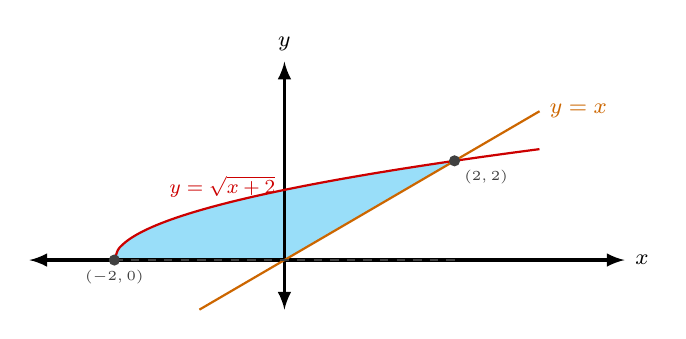
\begin{tikzpicture}[scale=0.9,x=1.2cm,y=0.7cm]
                \def\fx{sqrt(\x+2)}
                \def\gx{\x}
                %shading
                \fill[domain=-2:2,smooth,samples=100,variable=\x, cyan!40] plot ({\x},{\fx})--(0,0)--cycle;
                %axes
                \draw[latex-latex,very thick] (-3,0)--(4,0) node [right] {\footnotesize$x$};
                \draw[latex-latex,very thick] (0,-1)--(0,4) node [above] {\footnotesize$y$};
                %graphs
                \draw[domain=-2:3,smooth,samples=120,variable=\x, red!80!black, thick] plot ({\x},{\fx}) node [midway,above left,yshift=5ex] {\footnotesize$y=\sqrt{x+2}$};
                \draw[domain=-1:3,smooth,variable=\x, thick, orange!80!black] plot ({\x},{\gx}) node [right] {\footnotesize$y=x$};
                %intersection points
                \draw[fill=black,darkgray] (2,2) circle (2pt) node [below right] {\tiny$(2,2)$};
                \draw[fill=black,darkgray] (-2,0) circle (2pt) node [below] {\tiny$(-2,0)$};
                \draw[darkgray,dashed] (-2,0) -- (2,0);
            \end{tikzpicture}
        \end{center}
        Agar lebih mudah, gunakan integrasi terhadap \( y \) dengan mengubah fungsinya menjadi
        \begin{align*}
            y &= \sqrt{x+2} \Rightarrow x = y^2 - 2\\
            y &= x \Rightarrow x = y
        \end{align*}
        dan batas integrasi dari \( y = 0 \) sampai \( y = 2 \). Maka luas daerah yang diarsir dapat dihitung dengan integral berikut
        \begin{align*}
            \text{Area} &= \int_{0}^{2} \left( y - (y^2 - 2) \right) \, dy \\
            &= \int_{0}^{2} (2 + y - y^2) \, dy = \left[ 2y + \frac{1}{2}y^2 - \frac{1}{3}y^3 \right]_{0}^{2} \\
            &= \left( 2(2) + \frac{1}{2}(2)^2 - \frac{1}{3}(2)^3 \right) - 0 = 4 + 2 - \frac{8}{3} = 6 - \frac{8}{3} = \boxed{\frac{10}{3}}
        \end{align*}
        \item Titik potong kurva dengan sumbu-\( x \) terjadi ketika \( y = 0 \):
        \begin{align*}
            -x^2 + x &= 0 \\
            x(-x + 1) &= 0 \\
            x = 0 \quad&\vee\quad x = 1
        \end{align*}
        Ilustrasi daerah yang diarsir dapat dilihat di bawah ini
        \begin{center}
            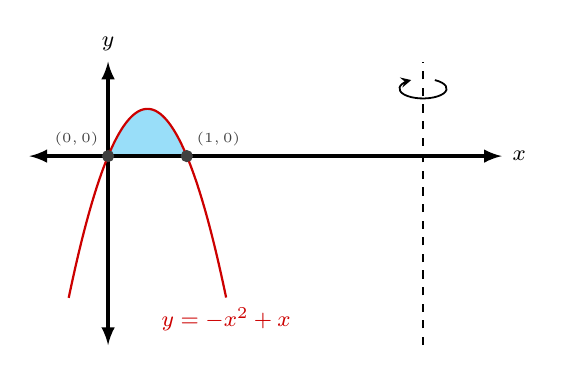
\begin{tikzpicture}[scale=2,y=1.2cm,x=0.5cm]
                \def\fx{-\x*\x+\x}
                %shading
                \fill[domain=0:1,smooth,samples=100,variable=\x, cyan!40] plot ({\x},{\fx})--(0,0)--cycle;
                %axes
                \draw[latex-latex,very thick] (-1,0)--(5,0) node [right] {\footnotesize$x$};
                \draw[latex-latex,very thick] (0,-1)--(0,0.5) node [above] {\footnotesize$y$};
                %graphs
                \draw[domain=-0.5:1.5,smooth,samples=120,variable=\x, red!80!black, thick] plot ({\x},{\fx}) node [below] {\footnotesize$y=-x^2+x$};
                %intersection points
                \draw[fill=black,darkgray] (1,0) circle (1pt) node [above right] {\tiny$(1,0)$};
                \draw[fill=black,darkgray] (0,0) circle (1pt) node [above left] {\tiny$(0,0)$};
                %Rotation axis
                \draw[thick,dashed] (4,-1) -- (4,0.5) node [midway,pos=0.9] {\AxisRotator[rotate=90]};
            \end{tikzpicture}
        \end{center}
        Karena diputar terhadap garis \( x = 4 \), maka kita perlu menghitung jarak titik berat dari garis tersebut yang dimana komponen yang dibutuhkan hanyalah \(\bar{x}\).\footnote{Ilustrasi pada gambar sebenarnya cukup menunjukkan bahwa daerah tersebut simetris terhadap $x=1/2$, sehingga dapat ditarik kesimpulan \(\bar{x} = 1/2\).}
        \begin{align*}
            M &= \int_{0}^{1} (-x^2+x) \, dx = \left[ -\frac{1}{3}x^3 + \frac{1}{2}x^2 \right]_{0}^{1} = \left( -\frac{1}{3}(1)^3 + \frac{1}{2}(1)^2 \right) - 0 = -\frac{1}{3} + \frac{1}{2} = \frac{-2+3}{6} = \frac{1}{6}\\
            M_y &= \int_{0}^{1} x(-x^2+x)\, dx = \int_{0}^{1} (-x^3+x^2) \, dx = \left[ -\frac{1}{4}x^4 + \frac{1}{3}x^3 \right]_{0}^{1} = \left( -\frac{1}{4}(1)^4 + \frac{1}{3}(1)^3 \right) - 0 \\
            &= -\frac{1}{4} + \frac{1}{3} = \frac{-3+4}{12} = \frac{1}{12}\\
            \bar{x} &= \frac{M_y}{M} = \frac{\frac{1}{12}}{\frac{1}{6}} = \frac{1}{2}
        \end{align*}
        Jadi $\Delta\bar{x} = |4 - \bar{x}| = 4 - \frac{1}{2} = \frac{8-1}{2} = \frac{7}{2}$. Kemudian gunakan rumus Dalil Guldin I untuk volume benda putar yaitu
        \[
            V = 2\pi L \Delta\bar{x} = 2\pi \left(\frac{1}{6}\right) \left(\frac{7}{2}\right) = \boxed{\frac{7\pi}{6}}
        \]
        \item Dapatkan turunan \( x \) dan \( y \) terhadap \( t \):
        \begin{align*}
            \frac{dx}{dt} &= 1 - \sin t \\
            \frac{dy}{dt} &= \cos t
        \end{align*}
        Kemudian gradien garis singgung pada \( t = 0 \) adalah
        \begin{align*}
            m &= \left.\frac{dy/dt}{dx/dt}\right|_{t=0} = \frac{\cos 0}{1 - \sin 0} = \frac{1}{1} = 1
        \end{align*}
        Untuk $t = 0$ juga diperoleh $x=1$ dan $y=2$. Sehingga persamaan garis singgung pada kurva tersebut adalah
        \begin{align*}
            y - 2 &= 1\cdot(x - 1) \\
            y &= x + 1
        \end{align*}
        \item Titik potong kedua kurva polar didapatkan dengan menyamakan kedua persamaan tersebut:
        \begin{align*}
            4\sin\theta &= 4\cos\theta \\
            \tan\theta &= 1 \\
            \theta &= \frac{\pi}{4}
        \end{align*}
        Sketsa daerah yang diarsir dapat dilihat di bawah ini
        \begin{center}
            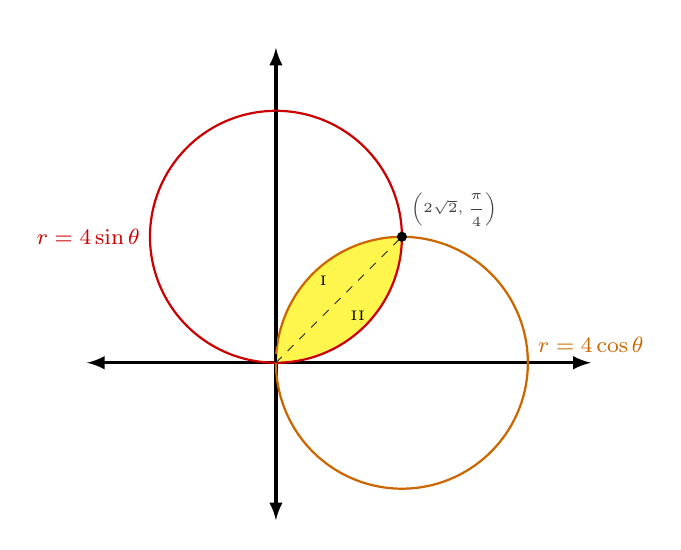
\begin{tikzpicture}[scale=0.8]
            \def\fr{4*sin(\o r)}
            \def\gr{4*cos(\o r)}
            %axes
            \draw[latex-latex,very thick] (-3,0)--(5,0) node [right] {};
            \draw[latex-latex,very thick] (0,-2.5)--(0,5) node [above] {};

            %shading
            \begin{scope}
                \clip[domain=0:pi/2,variable=\o] plot ({deg(\o)}:{\gr});
                \fill[domain=0:pi/2,smooth,samples=100,variable=\o, yellow!70] plot ({deg(\o)}:{\fr});
            \end{scope}

            %graphs
            \draw[domain=3*pi/4:7*pi/4,smooth,samples=120,variable=\o, red!80!black, thick] plot ({deg(\o)}:{\fr}) node [left] {\footnotesize$r=4\sin\theta$};
            \draw[domain=2*pi:0,smooth,samples=120,variable=\o, orange!80!black, thick] plot ({deg(\o)}:{\gr}) node [above right] {\footnotesize$r=4\cos\theta$};

            \draw[thick, dashed] (0,0) -- (0,4);
            \draw[darkgray, dashed] (0:0) -- ({deg(pi/4)}:{2*sqrt(2)}) node[above right] {\tiny$\left(2\sqrt{2}, \dfrac{\pi}{4}\right)$};
            \draw[fill=black] ({deg(pi/4)}:{2*sqrt(2)}) circle (2pt);

            \node at ({deg(pi/6)}:{1.5}) {\tiny II};
            \node at ({deg(pi/3)}:{1.5}) {\tiny I};
            \end{tikzpicture}
        \end{center}
        Perhatikan bahwa daerah I dan II adalah simetri, sehingga kita hanya perlu menghitung luas salah satu daerah saja kemudian mengalikan dengan 2.
        \begin{align*}
            \text{Area} &= 2\left[\frac{1}{2}\int_{0}^{\frac{\pi}{4}} (4\sin\theta)^2\, d\theta\right]\\
            &= \int_{0}^{\frac{\pi}{4}} 16\sin^2\theta \, d\theta\\
            &= \int_{0}^{\frac{\pi}{4}} 16\left(\frac{1-\cos 2\theta}{2}\right) \, d\theta\\
            &= 8\int_{0}^{\frac{\pi}{4}} \left(1-\cos 2\theta\right) \, d\theta\\
            &= 8\left[\theta - \frac{1}{2}\sin 2\theta\right]_{0}^{\frac{\pi}{4}}\\
            &= 8\left[\frac{\pi}{4} - \frac{1}{2}\sin \frac{\pi}{2}\right]= \frac{8\pi}{4} - 4 = \boxed{2\pi - 4}
        \end{align*}
        \item Cukup kita tinjau fungsi \( f(x) = xe^x \) dalam bentuk perkalian dari fungsi \( x \) dan \( e^x \).\footnote{Fungsi \( xe^x\) cukup sulit untuk diturunkan karena kita akan berhadapan dengan aturan perkalian.}
        Dapat kita gunakan deret Maclaurin untuk fungsi \( e^x \) yaitu\footnote{Untuk mencari deret Maclaurin dari fungsi \( e^x \), dapat kita gunakan turunan fungsi tersebut pada \( x = 0 \) }
        \[
            e^x = \sum_{n=0}^{\infty} \frac{x^n}{n!}
        \]
        Selanjutnya kalikan dengan \( x \) kedua fungsi tersebut:
        \[
            xe^x = x\sum_{n=0}^{\infty} \frac{x^n}{n!} = \sum_{n=0}^{\infty} \frac{x^{n+1}}{n!} 
        \]
        Dengan demikian, deret Maclaurin untuk $f(x) = xe^x$ adalah
        \begin{align*}
            f(x) &= \boxed{\sum_{n=0}^{\infty} \frac{x^{n+1}}{n!}} = x +x^2 + \frac{x^3}{2} + \frac{x^4}{6} + \cdots
        \end{align*}
    \end{enumerate}

    \newpage

    \pagestyle{problems}

    \begin{center}
	{\underline{\textbf{\MakeUppercase{Evaluasi Akhir Semester Bersama Genap 2023/2024}}}}
    \end{center}

    \begin{center}
	\begin{tabular}{lcl}
		Mata kuliah/SKS & : & Kalkulus 2 ( SM234201 ) / 3 SKS\\
		Hari, Tanggal & : & Kamis, 27 Juni 2024\\
		Waktu & : & 11.00-12.40 WIB (100 menit)\\
		Sifat & : & Tertutup\\
		Kelas & : & 48-60, 107
	\end{tabular}
    \end{center}
	
    \noindent\rule{\textwidth}{2.pt}
	
    \setlength{\parindent}{5pt}
    \par Diberikan 5 soal, dengan bobot nilai masing-masing soal sama dan boleh dikerjakan tidak berurutan.
    \setlength{\parindent}{5pt}
    \centering{Tuliskan: Nama, NRP, dan Nomor Kelas pada lembar jawaban Anda.}
    \setlength{\parindent}{5pt}
    {\small
    \par \textbf{\MakeUppercase{Dilarang membawa/menggunakan kalkulator dan alat komunikasi}}
    \centering{\textbf{\MakeUppercase{dilarang memberikan/menerima jawaban selama ujian}}}}
    \par \centering{\textbf{"Setiap tindak kecurangan akan mendapat sanksi akademik."}}
	
    \noindent\rule{\textwidth}{2.pt}
	
% SOAL DI SINI YAA
\begin{enumerate}
    \item Dapatkan luas daerah yang dibatasi oleh \( x = y^3 - y \) dan \( x = 0 \).

    \item Gambarkan daerah di kuadran I yang dibatasi oleh kurva-kurva \( y = x^2 \), \( y = 8 - 2x \), dan sumbu-\( y \). 
    Dapatkan volume benda putar jika daerah tersebut diputar pada sumbu-\( x \).

    \item Hitung panjang busur kurva 
    $
        x = a(t - \sin t), \quad y = a(1 - \cos t)
    $
    pada \( 0 \leq t \leq 2\pi \).\\
    Petunjuk: gunakan identitas trigonometri \( \cos 2t = 1 - 2\sin^2 t \).

    \item Dapatkan luas daerah yang diperoleh dari irisan kurva \( r = 3\cos \theta \) dan \( r = 1 + \cos \theta \).

    \item Dapatkan polinomial Taylor untuk fungsi \( f(x) = x \cos x \) di sekitar \( x = \pi \) hingga suku keempat.
\end{enumerate}
	
    \fancyfoot{
    \hrulefill\textbf{ Selamat Mengerjakan }\hrulefill

    \begin{center}
	    ``\textit{Jujur adalah kunci kesuksesan}''
    \end{center}}

    \newpage
    \pagestyle{solution}
    {\centering\textbf{SOLUSI}}

    \begin{enumerate}
      \item Titik potong kedua kurva diperoleh dari
      \begin{align*}
          y^3 - y &= 0 \\
          y(y^2 - 1) &= 0 \\
          y(y - 1)(y+1) &= 0 \\
          y = 0 \quad\vee\quad y &= 1 \quad\vee\quad y = -1
      \end{align*}
      
      Ilustrasi daerah dapat dilihat di bawah ini. 
      \begin{center}
          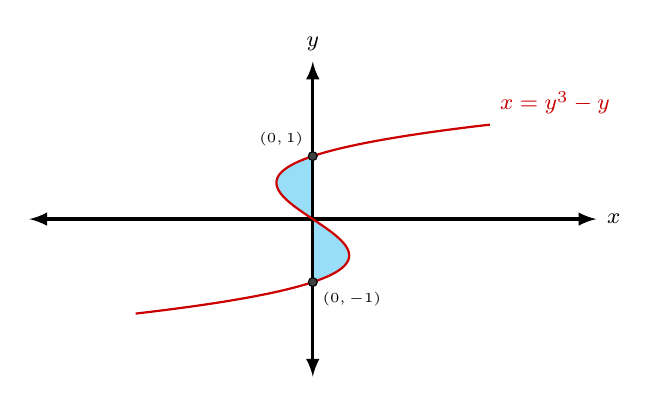
\begin{tikzpicture}[scale=0.8,x=1.5cm,y=1cm]
          \def\fy{\y*\y*\y-\y}
          %shading
          \fill[domain=-1:0,smooth,samples=100,variable=\y, cyan!40] plot ({\fy},{\y})--cycle;
          \fill[domain=0:1,smooth,samples=100,variable=\y, cyan!40] plot ({\fy},{\y})--cycle;

          %axes
          \draw[latex-latex,very thick] (-3,0)--(3,0) node [right] {\footnotesize$x$};
          \draw[latex-latex,very thick] (0,-2.5)--(0,2.5) node [above] {\footnotesize$y$};

          %graphs
          \draw[domain=-1.5:1.5,smooth,samples=120,variable=\y, red!80!black, thick] plot ({\fy},{\y}) node [above right] {\footnotesize$x=y^3-y$};

          %intersection points
          \draw[fill=darkgray] (0,1) circle (2pt) node[above left] {\tiny$(0,1)$};
          \draw[fill=darkgray] (0,-1) circle (2pt) node[below right] {\tiny$(0,-1)$};
          \end{tikzpicture}
        \end{center}
        Karena soal nya cukup ambigu, maka disini saya asumsikan bahwa daerah yang diarsir adalah daerah atas dan bawah seperti gambar di atas. Disebabkan kedua daerah simetris, maka cukup kita menghitung luas salah satu daerah saja kemudian mengalikan dengan 2.
        \begin{align*}
            \text{Area} &= 2\int_{0}^{1} -(y^3 - y) \, dy = 2\int_{0}^{1} (y - y^3) \, dy = 2\left[ \frac{1}{2}y^2 - \frac{1}{4}y^4 \right]_{0}^{1} = 2\left( \frac{1}{2} - \frac{1}{4} \right) = 2\left( \frac{1}{4} \right) = \boxed{\frac{1}{2}}
        \end{align*}
      \item Titik potong kedua kurva didapatkan dengan menyamakan kedua persamaan tersebut:
        \begin{align*}
            x^2 &= 8 - 2x \\
            x^2 + 2x - 8 &= 0 \\
            (x-2)(x+4) &= 0 \\
            x = 2 \quad&\vee\quad x = -4
        \end{align*}
        Ilustrasi daerah yang diarsir dapat dilihat di bawah ini
        \begin{center}
            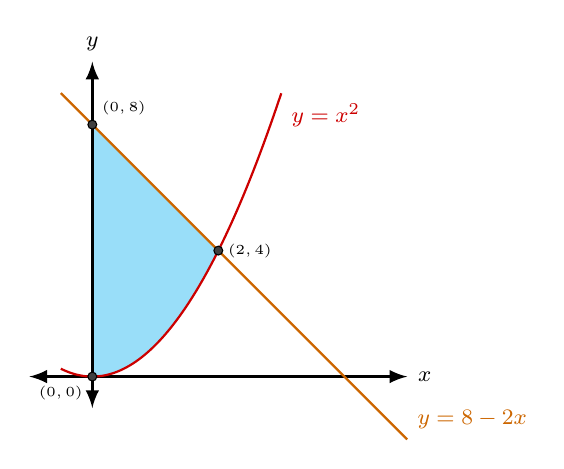
\begin{tikzpicture}[scale=0.8,x=1cm,y=0.5cm]
            \def\fx{\x*\x}
            \def\gx{8-2*\x}
            %shading
            \fill[domain=0:2,smooth,samples=100,variable=\x, cyan!40] plot ({\x},{\fx})-- (0,8) -- cycle;
            %axes
            \draw[latex-latex,very thick] (-1,0)--(5,0) node [right] {\footnotesize$x$};
            \draw[latex-latex,very thick] (0,-1)--(0,10) node [above] {\footnotesize$y$};

            %graphs
            \draw[domain=-0.5:3,smooth,samples=120,variable=\x, red!80!black, thick] plot ({\x},{\fx}) node [below right] {\footnotesize$y=x^2$};
            \draw[domain=-0.5:5,smooth,samples=120,variable=\x, orange!80!black, thick] plot ({\x},{\gx}) node [above right] {\footnotesize$y=8-2x$};

            %intersection points
            \draw[fill=darkgray] (2,4) circle (2pt) node [right] {\tiny$(2,4)$};
            \draw[fill=darkgray] (0,8) circle (2pt) node [above right] {\tiny$(0,8)$};
            \draw[fill=darkgray] (0,0) circle (2pt) node [below left] {\tiny$(0,0)$};
            \end{tikzpicture}
        \end{center}
        Selanjutnya, kita mencari $\bar{y}$ saja.
        \begin{align*}
            M &= \int_{0}^{2} (8 - 2x - x^2) \, dx = \left[ 8x - x^2 - \frac{1}{3}x^3 \right]_{0}^{2} = \left( 8(2) - (2)^2 - \frac{1}{3}(2)^3 \right) - 0 \\
            &= 16 - 4 - \frac{8}{3} = 12 - \frac{8}{3} = \frac{36-8}{3} = \frac{28}{3}\\
            M_x &= \frac{1}{2}\int_{0}^{2} (8 - 2x)^2-(x^2)^2 \, dx = \frac{1}{2}\int_{0}^{2} (64 - 32x + 4x^2 - x^4) \, dx \\
            &= \frac{1}{2}\left[ 64x - 16x^2 + \frac{4}{3}x^3 - \frac{1}{5}x^5 \right]_{0}^{2} = \frac{1}{2}\left( 128 - 64 + \frac{32}{3} - \frac{32}{5} \right)\\
            &= \frac{1}{2}\left( 64 + \frac{32}{3} - \frac{32}{5} \right) = \frac{1}{2}\left( \frac{960}{15} + \frac{160}{15} - \frac{96}{15} \right) = \frac{1}{2}\left( \frac{1024}{15} \right) = \frac{512}{15}\\
            \bar{y} &= \frac{M_x}{M} = \frac{\frac{512}{15}}{\frac{28}{3}} = \frac{512}{15} \cdot \frac{3}{28} = \frac{1536}{420} = \frac{256}{70} = \frac{128}{35}
        \end{align*}
        Terakhir menggunakan rumus Dalil Guldin I untuk volume benda putar yaitu
        \[
            V = 2\pi L \bar{y} = 2\pi \left(\frac{\cancelto{5}{28}}{3}\right) \left(\frac{128}{\cancelto{5}{35}}\right) = \boxed{\frac{512\pi}{15}}
        \]
      \item Turunkan $x$ dan $y$ terhadap $t$:
        \begin{align*}
            \frac{dx}{dt} &= a(1 - \cos t)\\
            \frac{dy}{dt} &= a\sin t
        \end{align*}
        Kemudian panjang busur kurva pada interval \( 0 \leq t \leq 2\pi \) adalah
        \begin{align*}
            L &= \int_{0}^{2\pi} \sqrt{\left(\frac{dx}{dt}\right)^2 + \left(\frac{dy}{dt}\right)^2} \, dt\\
            &= a\int_{0}^{2\pi} \sqrt{(1 - \cos t)^2 + (\sin t)^2} \, dt\\
            &= a\int_{0}^{2\pi} \sqrt{1 - 2\cos t + \cos^2 t + \sin^2 t} \, dt\\
            &= a\int_{0}^{2\pi} \sqrt{2 - 2\cos t} \, dt = a\int_{0}^{2\pi} \sqrt{2(1 - \cos t)} \, dt\\
            &= a\int_{0}^{2\pi} 4\sqrt{\sin^2(t/2)}\, dt= 4a\int_{0}^{2\pi} |\sin(t/2)|\, dt
        \end{align*}
        Karena \( |\sin(t/2)| = -\sin(t/2) \) pada interval \( [0,\pi] \) dan \( |\sin(t/2)| = \sin(t/2) \) pada interval \( [\pi, 2\pi] \), maka kita dapat memecah integral menjadi dua bagian:
        \begin{align*}
            S &= 4a\left(\int_{0}^{\pi} -\sin(t/2)\, dt + \int_{\pi}^{2\pi} \sin(t/2)\, dt\right)\\
            &= 4a\left(-2[\cos(t/2)]_{0}^{\pi} + 2[\cos(t/2)]_{\pi}^{2\pi}\right)\\
            &= 4a(-2[\cos(\pi/2)-1] + 2[1-\cos(3\pi/2)])\\
            &= 4a(-2[0-1] + 2[1-0])\\
            &= 4a(-2(-1) + 2(1)) = 4a(2 + 2) = \boxed{8a}
        \end{align*}
      \item Titik potong kedua kurva polar didapatkan dengan menyamakan kedua persamaan tersebut:
        \begin{align*}
            3\cos\theta &= 1 + \cos\theta \\
            2\cos\theta &= 1 \\
            \cos\theta &= \frac{1}{2} \\
            \theta = \frac{\pi}{3} \quad&\vee\quad \theta = -\frac{\pi}{3}
        \end{align*}
        Sketsa daerah yang diarsir dapat dilihat di bawah ini
        \begin{center}
            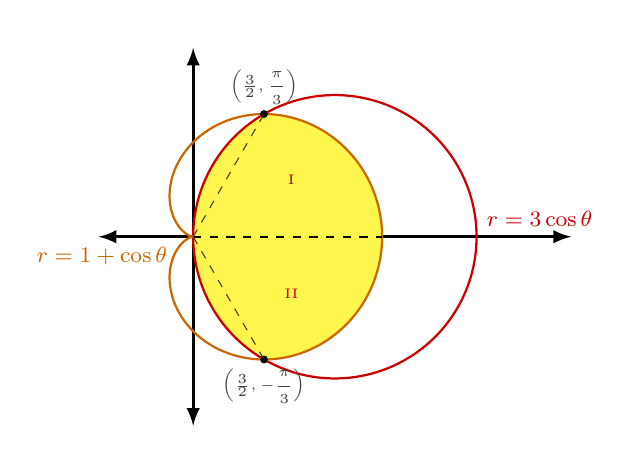
\begin{tikzpicture}[scale=1.2]
            \def\fr{3*cos(\o r)}
            \def\gr{1+cos(\o r)}
            %axes
            \draw[latex-latex,very thick] (-1,0)--(4,0) node [right] {};
            \draw[latex-latex,very thick] (0,-2)--(0,2) node [above] {};

            %shading
            \begin{scope}
                \clip[domain=0:2*pi,smooth,samples=100,variable=\o] plot ({deg(\o)}:{\fr});
                \fill[domain=0:2*pi,smooth,samples=100,variable=\o, yellow!70] plot ({deg(\o)}:{\gr});
            \end{scope}

            %graphs
            \draw[domain=0:2*pi,smooth,samples=120,variable=\o, red!80!black, thick] plot ({deg(\o)}:{\fr}) node [above right] {\footnotesize$r=3\cos\theta$};
            \draw[domain=-pi:pi,smooth,samples=120,variable=\o, orange!80!black, thick] plot ({deg(\o)}:{\gr}) node [below left,xshift=-0.2cm] {\footnotesize$r=1+\cos\theta$};

            \draw[thick,dashed] (0,0) -- (2,0);

            %intersection points
            \draw[darkgray,dashed] (0:0) -- ({deg(pi/3)}:{3/2}) node[above] {\tiny$\left(\frac{3}{2}, \dfrac{\pi}{3}\right)$};
            \draw[fill=black] ({deg(pi/3)}:{3/2}) circle (1pt);
            \draw[darkgray,dashed] (0:0) -- ({-deg(pi/3)}:{3/2}) node[below] {\tiny$\left(\frac{3}{2}, -\dfrac{\pi}{3}\right)$};
            \draw[fill=black] ({-deg(pi/3)}:{3/2}) circle (1pt);

            \node[purple] at ({deg(pi/6)}:{1.2}) {\tiny I};
            \node[purple] at ({-deg(pi/6)}:{1.2}) {\tiny II};
            \end{tikzpicture}
        \end{center}
        Perhatikan bahwa daerah I dan II adalah simetri, sehingga kita hanya perlu menghitung luas salah satu daerah saja kemudian mengalikan dengan 2.

        Tinjau juga bahwa salah satu daerah dapat dihitung sebagai 2 integral polar terpisah, yaitu
        \[ \frac{1}{2}\int_{0}^{\frac{\pi}{3}} \left(1+\cos\theta\right)^2 \, d\theta \quad\text{dan}\quad \frac{1}{2}\int_{\frac{\pi}{3}}^{\frac{\pi}{2}} \left(3\cos\theta\right)^2 \, d\theta \]
        Maka luas daerah yang diarsir dapat dihitung dengan integral berikut
        \begin{align*}
            \text{Area} &= 2\left[\frac{1}{2}\int_{0}^{\frac{\pi}{3}} \left(1+\cos\theta\right)^2 \, d\theta + \frac{1}{2}\int_{\frac{\pi}{3}}^{\frac{\pi}{2}} (3\cos\theta)^2 \, d\theta\right]\\
            &= \int_{0}^{\frac{\pi}{3}} (1+\cos\theta)^2 \, d\theta + \int_{\frac{\pi}{3}}^{\frac{\pi}{2}} 9\cos^2\theta \, d\theta\\
            &= \int_{0}^{\frac{\pi}{3}} (1 + 2\cos\theta + \cos^2\theta) \, d\theta + 9\int_{\frac{\pi}{3}}^{\frac{\pi}{2}} \left(\frac{1+\cos 2\theta}{2}\right) \, d\theta\\
            &= \left[\frac{3}{2}\theta + 2\sin\theta + \frac{1}{4}\sin 2\theta\right]_{0}^{\frac{\pi}{3}} + 9\left[\frac{1}{2}\theta + \frac{1}{4}\sin 2\theta\right]_{\frac{\pi}{3}}^{\frac{\pi}{2}}\\
            &= \left[\frac{\cancel{3}}{2}\cdot\frac{\pi}{\cancel{3}} + 2\left(\frac{\sqrt{3}}{2}\right) + \frac{1}{4}\left(\frac{\sqrt{3}}{2}\right)\right] - 9\left[\frac{1}{2}\cdot\frac{\pi}{2} + \frac{1}{4}\cdot 0 - \left(\frac{1}{2}\cdot\frac{\pi}{3} + \frac{1}{4}\cdot\left(\frac{\sqrt{3}}{2}\right)\right)\right]\\
            &= \left[\frac{\pi}{2} + \frac{9\sqrt{3}}{8}\right] + 9\left[\frac{\pi}{12} - \frac{\sqrt{3}}{8}\right]\\
            &= \frac{\pi}{2} + \frac{9\sqrt{3}}{8} + \frac{3\pi}{4} - \frac{9\sqrt{3}}{8}= \boxed{\frac{5\pi}{4}}
        \end{align*}
      \item Mencari turunan fungsi pertama sampai keempat dari fungsi \( f(x) = x \cos x \):
        \begin{align*}
            f'(x) &= \cos x - x\sin x\\
            f''(x) &= -\sin x - \sin x - x\cos x = -2\sin x - x\cos x\\
            f'''(x) &= -2\cos x - \cos x + x\sin x = -3\cos x + x\sin x\\
            f^{(4)}(x) &= 3\sin x + \sin x + x\cos x = 4\sin x + x\cos x 
        \end{align*}
        Kemudian substitusi \( x = \pi \):
        \begin{align*}
            f(\pi) &= \pi(-1) = -\pi\\
            f'(\pi) &= -1 - \pi(0) = -1\\
            f''(\pi) &= -2(0) - \pi(-1) = \pi\\
            f'''(\pi) &= -3(-1) + \pi(0) = 3\\
            f^{(4)}(\pi) &= 4(0) + \pi(-1) = -\pi
        \end{align*}
        Maka polinomial Taylor untuk $f(x)$ di sekitar $x=\pi$ hingga suku keempat adalah
        \begin{align*}
            &P_4(x) = f(\pi)+f'(\pi)(x-\pi)+\frac{f''(\pi)}{2!}(x-\pi)^2+\frac{f'''(\pi)}{3!}(x-\pi)^3+\frac{f^{(4)}(\pi)}{4!}(x-\pi)^4\\
            &\boxed{P_4(x) = -\pi - (x-\pi) + \frac{\pi}{2}(x-\pi)^2 + \frac{1}{2}(x-\pi)^3 - \frac{\pi}{24}(x-\pi)^4}
        \end{align*}
    \end{enumerate}
    
\end{document}